%&latex
% UF Sample ETD Main Document Fall 2014
% Documenting the dvipdfmx/dvipdfm "File not Found" error
% Improved method of handling the single/multiple appendices issue
% Updated font calls to meet latest LaTeX standards

% Define Document Class to be used and options - Choose the option that meets your OS%
%\documentclass[12pt,dvipdfm,final,CPage]{ufthesis} %Use this line for Windows OS
\documentclass[12pt,dvipdfmx,final,CPage]{ufthesis} %Use this line for Macintosh/Linux OS



% Macintosh and Linux users - If you get a dvipdfm file not found error
% change dvipdfm to dvipdfmx here and in the packages.tex file graphicx and hyperref packages and
% compile using Latex, Latex, Bibtex, Latex, Latex, XeLaTeX - this usually fixes
% the problem NOTE: If you are including an Appendix Latex will complain about
% "something missing" press "r" followed by "Enter" and Tex will ignore the error.

%-------------------------------------C:\Program Files\MiKTeX 2.5\miktex----------------------------------%
% Preamble %

% Define Packages To be used and options %
% here you define all the packages you wish to use in your paper, the ones shown are not all necessary,
% but all have purpose and can be very useful, so leave these as default and add packages as necassary
\usepackage[dvipdfmx]{graphicx}
\usepackage{amsmath}
\usepackage{amsthm}
\usepackage{algpseudocode}
\usepackage{tabularx}
\usepackage{url}
\usepackage[letterpaper,hmargin=1in,vmargin=1in]{geometry}
\usepackage{lscape}
\usepackage{hanging}
\usepackage{longtable}
\usepackage{amsfonts}
\usepackage{amssymb}
%\usepackage[cmbright]{sfmath} % Comment this line to use Times New Roman Math Typeface
\usepackage{subfigure}
\usepackage{rotating}
\usepackage{calc}
\usepackage{setspace}
\usepackage{ufenumerate}
\usepackage{latexsym}
\usepackage{epsf}
\usepackage{epsfig}
\usepackage{euscript}
\usepackage[format=hang,justification=raggedright,singlelinecheck=0,labelsep=period]{caption}
%\usepackage[numbers,sort&compress]{natbib} %Use this set-up for numbered reference lists
\usepackage[authoryear]{natbib} %Use this set-up if you want an un-numbered reference list     http://merkel.zoneo.net/Latex/natbib.php
%\usepackage{hypernat}




\usepackage[dvipdfmx,hyperfootnotes=false]{hyperref}
%\usepackage[dvips,hyperfootnotes=false]{hyperref}
%\hypersetup{colorlinks=true,linkcolor=blue,anchorcolor=blue,citecolor=blue,filecolor=blue,urlcolor=blue,bookmarksnumbered=true,pdfview=FitB} %
\hypersetup{colorlinks=true,linkcolor=black,anchorcolor=black,citecolor=black,filecolor=black,urlcolor=black,bookmarksnumbered=true,pdfview=FitB} %

% % %DO NOT PLACE ANY PACKAGES AFTER THE HYPERREF SET UP


\def\UrlFont{\rmfamily} %use this line for Times New Roman
%\def\UrlFont{\sffamily} %use this line for Helvetica

%\allowdisplaybreaks  % % This command allows equation arrays and similar environments
% % % to break across pages to improve text flow - use only if needed.

% Prevent figures, tables or algorithms from using a separate page or column alone
\renewcommand{\topfraction}{0.85}
\renewcommand{\textfraction}{0.1}
\renewcommand{\floatpagefraction}{0.75}

% *** Do not adjust lengths that control margins, column widths, etc. ***
% *** Do not use packages that alter fonts (such as pslatex).         ***
% There should be no need to do such things with IEEEtran.cls V1.6 and later.
% correct bad hyphenation here
%\hyphenation{op-tical net-works semi-C:\Program Files\MiKTeX 2.5\miktexconduc-tor}

%------------------------------------------%

% Extra commands or misc formatting such as page alignment or output paper-size commands

%\include{extraparameters}

%------------------------------------------%

% Set your personal and paper information
\SetFullName{Morteza Shahriari Nia}%
\SetThesisType{Dissertation}%{Tutorial}% %{Thesis}
\SetDegreeType{Doctor of Phylosophy}% {Doctor of Philosophy} {Master of Science}
\SetGradMonth{April}%
\SetGradYear{2015}%
\SetDepartment{Electronics and Computer Engineering}%
\SetChair{Dr. Daisy Zhe Wang}%
%\SetCochair{John W. Carver III}%uncomment this line and enter the name of your cochair inside the braces if you have one.
%If you have a cochair there two places in the ufthesis.cls file that will need to be uncommented as well
%In the "getting personal information" section about line 630
%And the "Abstract" Section around line 556
% Type your title here in all CAPS %
\SetTitle{Big Data in Ecology}



% Define student-specific info (self-explanatory) %
%\include{userinfo}






%------------------------------------------%

% user defined commands in order to geC:\Program Files\MiKTeX 2.5\miktexnerate new commands, macros, and redefine default commands %
% user defined commands %
% Here is where you define optional commands such as macros, new commands,
% and new environments to be used in your paper

% optional command to prevent a word from breaking across a line %
\hyphenchar\font=-1


% Commands to produce proper bullet list
\newlength{\widthOfItem}
\let\Itemize=\itemize
\let\endItemize=\enditemize
\renewenvironment{itemize}{%
	\begin{Itemize}
		\setlength{\itemsep}{0.5\baselineskip}
		\setlength{\labelwidth}{2em}
		\setlength{\listparindent}{.32in}%
		\setlength{\leftmargin}{.32in}
		\setlength{\rightmargin}{0in}
		\settowidth{\widthOfItem}{\labelitemi}
		\setlength{\labelsep}{\leftmargin-\widthOfItem}
		\renewcommand{\labelitemii}{--}
		\singlespacing}{%
	\end{Itemize}}

% shortcut for setting up inserting \prime command in mathmode to avoid errors %
\newcommand{\p}{^{\prime}}

% shortcuts for prime color text
\newcommand{\red}{\textcolor[rgb]{1.00,0.00,0.00}}
\newcommand{\green}{\textcolor[rgb]{0.00,1.00,0.00}}
\newcommand{\blue}{\textcolor[rgb]{0.00,0.00,1.00}}

% Shorcut commands for mathmatical formulas %

\newcommand{\latex}{\LaTeX 2\ensuremath{\epsilon}}

% THEOREM Environments ---------------------------------------------------
%These environments are provided as a convenience - feel free to modify if needed

\newtheorem{theorem}{Theorem}[chapter]%To link the theorem to each chapter uncomment the chapter option
\newtheorem{lemma}{Lemma}%[theorem]% To link each lemma to a theorem uncomment the theorem option
\newtheorem{corollary}{Corollary}%[theorem]% To link each corollary to a theorem uncomment the theorem option
% to link a corollary to a chapter change the theorem option to chapter
\newtheorem{definition}{Definition}%[chapter] %the same is true for both definitions and assumptions
\newtheorem{assumption}{Assumption}%[chapter] %
\newtheorem{proposition}{Proposition}[chapter]


%These were some user commands I've run across that I thought some might want to incorporate into their work
%\newcommand{\bdm}{
 %   \begin{displaymath}}

%\newcommand{\edm}{
%    \end{displaymath}}

%\newcommand{\be}{
%    \begin{equation}}

%\newcommand{\ee}{
%    \end{equation}}

%\newcommand{\bea}{
 %   \begin{eqnarray}}

%\newcommand{\eea}{
%    \end{eqnarray}}


%-------------------------------------------------------------------------------------------------------%

% Begin Main Part of Document %

\begin{document}


 % % % % % % % % % % % % % % % % % % % % % % % % % % % % % % % % % % % % % %
 % Remember - You MUST get a .bst file that matches the Journal in your
 % field that you choose as your Reference example
 % NONE of these examples will satisfy the Graduate Editorial Office
 % if they don't match your Journal example!!!!
 % NOTE: If you use a numbered reference system and your references
 % are set in parentheses rather than brackets you need to select the
 % Natbib option "numbers sort and compress" in the packages.tex file
 % % % % % % % % % % % % % % % % % % % % % % % % % % % % % % % % % % % % % %


 %Note that the path separator is a forward slash NOT a back slash
 %Place YOUR .bst file in the bst folder and use that filename (without the .bst extension)
 % as your Bibliography Style file

%\bibliographystyle{bst/abbrv}
%\bibliographystyle{bst/abbrvnat}
%\bibliographystyle{bst/abbrvurl_uf}
%\bibliographystyle{bst/alphaurl_uf}
%\bibliographystyle{bst/apa-good}
%\bibliographystyle{bst/Chicago_Web}
%\bibliographystyle{bst/ecology_web}
%\bibliographystyle{bst/IEEEtran}
%\bibliographystyle{bst/mla_web}
\bibliographystyle{bst/mla-good}
%\bibliographystyle{bst/plainnat}
%\bibliographystyle{bst/plainurl_uf}
%\bibliographystyle{bst/Science_Web}
%\bibliographystyle{bst/uf_econ}
%\bibliographystyle{bst/uffull}
%\bibliographystyle{bst/ufinit}
%\bibliographystyle{bst/unsrtnat}
%\bibliographystyle{bst/unsrturl_uf}
%\bibliographystyle{bst/plain}
%\bibliographystyle{bst/ufinit}
%\bibliographystyle{bst/plainurl_uf}


%-----------------------------------------------------------------------%

\maketitle % % % % Creates the Title page from the information entered in userinfo.tex
\makecopyright

%------------------------------------------%

\dedication{% Add your text for the dedication here between the center tags
\addvspace{4.25in}
\begin{center}\singlespacing
I dedicate this to my parents who selflessly devoted the best of their lives to raise their kids to be hard working, humble, selfless and to take steps towards \\the greater human wisdom\\
\end{center}
} % %Creates the dedication - if your dedication is more than a single line
% % % % % % % % % % % % % % % % % %you will need to reduce the vspace amount to keep the text centered verticlly
% % % % % % % % % % % % % % % % % %optional - comment or delete if you are not dedicating to anyone,

%------------------------------------------%

% Make sure to keep the text within the brackets and the output should turn out correct
\acknowledge{%
I would like to thank Dr. Daisy Zhe Wang for believing in me and providing the great opportunity of tackling the whole real of big data. I would also like to thank Dr. Yuguang Fang for his great support and commitment. Dr. Paul Gader and Dr. Stephanie Bohlman were great mentors, without contributions of whom this work would not have been possible. }
 % % % %Required - There is no requirement to acknowledge a particular person
% % % % % % % % % % % % % % % % %but you must acknowledge someone (funding source, committee chair, spouse)?

%------------------------------------------%

% This file includes the file which creates the table of contents %
% This creates your table of contents, list of figures, and list of tables
% the pdfbookmark line adds the word to the bookmarks of the pdf without adding it to the TOC itself
\pdfbookmark[0]{TABLE OF CONTENTS}{tableofcontents}
\tableofcontents %
\listoftables %
%\setcounter{lofdepth}{2}
\listoffigures %

% Produced list of abbreviations or symbols %
%\printindex[keylist]{KEY TO ABBREVIATIONS}{KEY TO ABBREVIATIONS}{}
%\printindex[mathlist]{KEY TO SYMBOLS}{KEY TO SYMBOLS}{%
%The list shown below gives a brief description of the major mathematical symbols defined in this work. For each
%symbol, the page number corresponds to the place where the symbol is first used.} %
 %This file creates the Table of Contents, List of Figures, and List of Objects (if any)
% % % % % % % %delete or comment the file you want to remove

%------------------------------------------%

%%This is an optional file. A list of abbreviations is NOT even suggested.
%%Best practice is to define the item the first time it is used in the document

%%%-----------List of Symbols, Nomenclature or Abbreviation--------

%% Please note: a list of Symbols, terms, acronyms, etc. is not usually the best practice.
%% More often you should simply define an abbreviation the first time it is used.
%% If you DO need to include a list like this please notice that it must be paginated manually
%% by breaking it up into page size tables. Longtable will not wrap the definition properly if
%% it extends to a second line and a similar issue is encountered when the tabbing environment
%% is used. If you have a better way of meeting the Editorial Office requirements I'd love to hear about it.

\chapter*{LIST OF SYMBOLS, NOMENCLATURE, OR ABBREVIATIONS} \addcontentsline{toc}{chapter}{LIST OF SYMBOLS} %Start
%writing here. This is optional.
\singlespacing
\begin{tabular}{l p{5in}} %if the terms in the first column are longer than 1.4 inches reduce the number 5 appropriately
$\sum$ & Denotes the summation of a series of terms\\
\\%This adds the single space between definitions (required)
$\bigcap$ & A really big bigcap\\
\\
fractal & A geometric pattern that is repeated at ever smaller
scales to produce irregular shapes and surfaces that cannot be represented by classical
geometry. Fractals are used especially in computer modeling of irregular patterns and structures in nature.}\\
\\
polynomial & (in one variable) an expression consisting of the sum of two
or more terms each of which is the product of a constant and a
variable raised to an integral power: $ax^2 + bx + c$ is a
polynomial, where $a, b,$ and $c$ are constants and $x$ is a
variable.}\\
\\
$\sum$ & Denotes the summation of a series of terms\\
\\
$\bigcap$ & A really big bigcap\\
\\
fractal & A geometric pattern that is repeated at ever smaller
scales to produce irregular shapes and surfaces that cannot be represented by classical
geometry. Fractals are used especially in computer modeling of irregular patterns and structures in nature.}\\
\\
polynomial & (in one variable) an expression consisting of the sum of two
or more terms each of which is the product of a constant and a
variable raised to an integral power: $ax^2 + bx + c$ is a
polynomial, where $a, b,$ and $c$ are constants and $x$ is a
variable.}\\
\\
$\sum$ & Denotes the summation of a series of terms\\
\\
$\bigcap$ & A really big bigcap\\
\\
fractal & A geometric pattern that is repeated at ever smaller
scales to produce irregular shapes and surfaces that cannot be represented by classical
geometry. Fractals are used especially in computer modeling of irregular patterns and structures in nature.}\\
\\
polynomial & (in one variable) an expression consisting of the sum of two
or more terms each of which is the product of a constant and a
variable raised to an integral power: $ax^2 + bx + c$ is a
polynomial, where $a, b,$ and $c$ are constants and $x$ is a
variable.}\\

\end{tabular}

\begin{tabular}{lp{5in}}
$\sum$ & Denotes the summation of a series of terms\\
\\
$\bigcap$ & A really big bigcap\\
\\
fractal & A geometric pattern that is repeated at ever smaller
scales to produce irregular shapes and surfaces that cannot be represented by classical
geometry. Fractals are used especially in computer modeling of irregular patterns and structures in nature.}\\
\\
polynomial & (in one variable) an expression consisting of the sum of two
or more terms each of which is the product of a constant and a
variable raised to an integral power: $ax^2 + bx + c$ is a
polynomial, where $a, b,$ and $c$ are constants and $x$ is a
variable.}\\
\\
$\sum$ & Denotes the summation of a series of terms\\
\\
$\bigcap$ & A really big bigcap\\
\\
fractal & A geometric pattern that is repeated at ever smaller
scales to produce irregular shapes and surfaces that cannot be represented by classical
geometry. Fractals are used especially in computer modeling of irregular patterns and structures in nature.}\\
\\
polynomial & (in one variable) an expression consisting of the sum of two
or more terms each of which is the product of a constant and a
variable raised to an integral power: $ax^2 + bx + c$ is a
polynomial, where $a, b,$ and $c$ are constants and $x$ is a
variable.}\\
\\
$\sum$ & Denotes the summation of a series of terms\\
\\
$\bigcap$ & A really big bigcap\\
\\
fractal & A geometric pattern that is repeated at ever smaller
scales to produce irregular shapes and surfaces that cannot be represented by classical
geometry. Fractals are used especially in computer modeling of irregular patterns and structures in nature.}\\
\\
polynomial & (in one variable) an expression consisting of the sum of two
or more terms each of which is the product of a constant and a
variable raised to an integral power: $ax^2 + bx + c$ is a
polynomial, where $a, b,$ and $c$ are constants and $x$ is a
variable.}\\
\\
\end{tabular}
\doublespacing




%------------------------------------------%
% This line adds the word CHAPTER to the TOC just before the listing of the chapter and subsections begins
\addtocontents{toc}{\protect\addvspace{10pt}\noindent{CHAPTER}\protect\hfill\par}{}% This extra line adds the word CHAPTER to the table of contents %
\phantomsection
% Write in only the text of your abstract, all the extra heading jargon is automatically taken care of
\begin{abstract}
This document is the official tutorial outlining the use and
implementation of the UF \LaTeX 2\ensuremath{\epsilon} Template for
use on thesis and dissertations. The tutorial will cover the basic
files, commands, and syntax in order to properly implement the
template.  It should be made clear that this tutorial will not tell
one how to use \LaTeX 2\ensuremath{\epsilon}.  It will be assumed
that you will have had some previous knowledge or experience with
\LaTeX 2\ensuremath{\epsilon}, but, there are many aspects of publishing 
for the UF Graduate School that requires attention to some details that are 
normally not required in \LaTeX 2\ensuremath{\epsilon}.

Pay particular attention to the section on references. NONE of the bibliography style files (.bst) are an assurance that your document's reference style will meet the Editorial Guidelines. You MUST get a .bst file that matches the style used by the journal you used as a guide for your references and citations. The files included in this document are examples only and are NOT to be used unless they match your sample article exactly!

You should have a .bib file (we have included several examples) that contains your reference sources. Place your .bib file in the bib folder and enter the name of the file in the list of bib files, or enter your reference information into one of our existing .bib files if you don't already have one. Just make sure to preserve the format of each kind of reference. Each time you cite a reference you enter the "key" (the first field in the reference listing in the .bib file) associated with that reference. During the compilation process LaTeX will gather all the references, insert the correct method of citation and list the references in the correct location in the proper format for the reference style selected.
\end{abstract}
 %The abstract is created using this file and userinfo.tex
% % % % % % % % % % %If you have a c-chair you must uncomment that line in userinfo.tex AND find the
% % % % % % % % % % %co-chair lines in ufthesis.cls and un-comment those as well

%-----------------------------------------------------------------------%

% This section encompasses the main body of the paper from all the content through to the biographical sketch

% Chapters to be included (more can be added by creating a new chapter#.tex %
% file and then implementing the \inlcude{chapter#.tex} command as seen below %
\chapter{Introduction}%

Understanding the dynamics of ecological structures is very important in determining how climate, %CO\textsuperscript{2} emission, 
land cover %(water resources, desertification)
, fire hazards, and biodiversity evolve. Precision study of plant species is of high environmental and economical impacts which is only possible through geo-mapping the distribution of plant species abundances at ecological scale. Large scale study of ecological domains has been made possible through spaceborne or airborne campaigns utilizing remote sensing technologies such as \textit{(multi/hyper)-spectral} and \textit{LiDAR}. In this project we focus on airborne hyperspectral and LiDAR data. Each campaign covering tens of acres of land can generate terra-bytes of data depending on measurement resolution (large volume). On the other hand, apart from state-of-the-art machine learning algorithms, there is a great wealth of expert ecological knowledge covering a whole variety of domains (along with their in-ground associated data) that can be used to enhance species mapping that is not being used and is left for ecological scientists for manual interpretation (data variety). Furthermore, data is being generated at faster pace day after day as technology becomes more afordable. After satellite sensors, airborne sensors came into place and now as airborne is still costly there is a surge of interest towards more affordable drone campaigns \citep{zhou2009foreword}. So we are facing data being generated at unprecedented rates (data velocity). The final aspect is verasity: imperfect sensors, non-standardized measurements, atmosphere impacts (clouds, humidity, aerosols) and et cetera all create uncertainities that need to be accounted for. Velocity, verasity, volume, and variety are the four V's that indicate ecology is stepping into the realm of "big data"\citep{hampton2013big, soranno2014macrosystems}.

\section{Remote Sensing}

From an ecological point of view, there are two types of remote sensing approaches: active and passive. \textit{Passive} remote sensing uses sunlight as the source of energy and sensors captures the intensity of light being reflected from earth's surface. Light intensity measurements happens at various wavelengths; if a few (usually 3 to 10) relatively broad wavelength bands are captured it is called multi-spectral. If light intensity at dozens to hundreds of narrow band signals are collected it is called hyperspectral. \textit{Active} remote sensing on the other hand uses laser light emission as its source of energy and captures the intensity of returned signals. LiDAR is a popular active remote sensing technology. Below we explain each in more details:



\subsection{Hyperspectral}

\begin{figure}[b!]
  \centering
    \includegraphics[scale=0.22]{images/spectrometer.eps}
    \caption[Imaging spectrometer schematic diagram]{Schematic diagram of the basic elements of an imaging spectrometer where $\lambda$ is the wavelength \citep{smith2006introduction}.}
    \label{fig:Imaging spectrometer}
\end{figure}

Spectrometers measure the amount of light reflected from surface materials: An optical dispersing element (like a prism) refracts the received light into its constituent spectrums and the energy in each band range is measured by a separate detector. Bands can be as narrow as $0.01 \mu m$ over a wide wavelength range of typically $0.4 \mu m$ to $2.5 \mu m$. Figure~\ref{fig:Imaging spectrometer} shows the basic components of an imaging spectrometer.

Raw sensor readings (digital number) can be affected by light source conditions, sensor, atmosphere, and surface material. Raw data which is a unit-less light intensity measure is then calibrated into radiance which has a  physically meaningful unit through applying a gain and offset to the pixel values. It essentially means how much light the instrument ''sees'' from the object being observed. Some reference materials like a pure white or pure black sheets can be used in this process. After adjustments for sensor, atmospheric, and terrain effects are applied, pixel reflectance value is calculated which is the proportion of the radiation striking a surface to the radiation reflected off of it. Reflectance demonstrates light abroption features of the surface material and can be compared with field or laboratory reflectance spectra in order to recognize and map surface materials such as particular types of vegetation or diagnostic minerals associated with ore deposits. Reflectance varies with wavelength for most materials because energy at certain wavelengths is scattered or absorbed to different degrees \citep{smith2006introduction}. In this project we deal with reflectance values and refer the reader to \citep{varshney2004advanced} for more details on how to compute reflectance values.


\begin{figure}[t!]
  \centering
    \includegraphics[scale=0.45]{images/reflectanceAsIndicator.eps}
    \caption[Some reflectance examples]{Some reflectance examples as how reflectance of different material show different absroption features at differnet bands. \citep{smith2006introduction}.}
    \label{fig:Some reflectance examples}
\end{figure}

Figure~\ref{fig:Some reflectance examples} shows some example materials when observed through an spectrometer. In vegetations, chlorophyll and some leaf pigments show high absorptions in blue and red ranges and not so much in green; therefore our eyes see vegetation as green. We can see this as a small peak in green compared to other visible wavelength range. From red to near infrared there is a sharp rise known as \textit{red edge} up to a value of about 50\% for some plants. High values in the near-infrared region is mainly due to internal cellular structure of leaves which differs significantly across species but can also be different in a single specie due to plant stress. High reflectance in near-infrared can interact with other leaves in the canopy and therefore its sensor readings can be dependent on canopy structure as well. Beyond  $1.3 \mu m$ reflectance decreases with increasing wavelength, except for two pronounced water absorption bands near $1.4 \mu m$ and  $1.9 \mu m$. At the end of the growing season leaves lose water and chlorophyll. Near infrared reflectance decreases and red reflectance increases, creating the yellow, brown, and red leaf colors of autumn \citep{smith2006introduction}.

One note worthy concept is the issue of mixing. Pixel size can be large based on the distance between the sensor and target; this makes it likely that more than one material contribute to the signal received by the sensor. The received signal is called a \textit{composite} or \textit{mixed} signal and the ''pure'' signal that contribute to the mixture are called \textit{endmember} signal. The mixture model can be either linear or non-linear. Linear mixture happens at macro-scale where we have for example a large patch of land beside a large patch of vegetation. If we denote the received signal, land, and vegetation as $S$,$L$, and $V$ respectively the mixture model could be  $S=60\%L+40\%V$. Linear mixture of three endmembers can easily be shown to fall within the triangle where its vertices are endmember spectra. Variations in lighting can be included directly in the mixing model by defining a ''shade'' endmember (shade, deep water body, dark asphalt or etc) that can approximate light changes and mix with the actual material spectra. Non-linear mixture model on the other hand is more intimate and happens at micro-scale. For example in a microscopic mixture of mineral particles found in soil, a single photon can interacts with more than one material, therefore resulting in a non-linear mixture \citep{keshava2003survey, bioucas2012hyperspectral, dobigeon2014nonlinear}.


\subsection{LiDAR}

Light Detection And Ranging (LiDAR) is a form of active remote sensing where a laser beam is used to detect points on earth. LiDAR sensor is mounted on an airplane and it keeps swiping earth surface as the plane moves forward. By knowing parameters of the LiDAR sensor itself (tilt angle of the pulse), plane GPS coorinates, and Inertial Measurement Unit (IMU) coordinates (heading, pitch and roll) and the speed of light, the exact coorinate of each point reading is calculated. LiDAR scans at pulse rates of over 300,000 pulses per second (300 kilohertz) depending on sensor technology. By subtracting plane altitude from the distance that laser has traveled we get the ground elevation.  Using some filtering techniques points on the ground are classified from points above the ground and this yeilds the height of the objects on the ground. Figure~\ref{fig:lidar} (A) demonstrates a schematic view of a LiDAR flightand its parameters \citep{schmid2008lidar}.


\begin{figure}[b!]
  \begin{center}
    \centering
    \mbox{
      \subfigure[]{\fbox{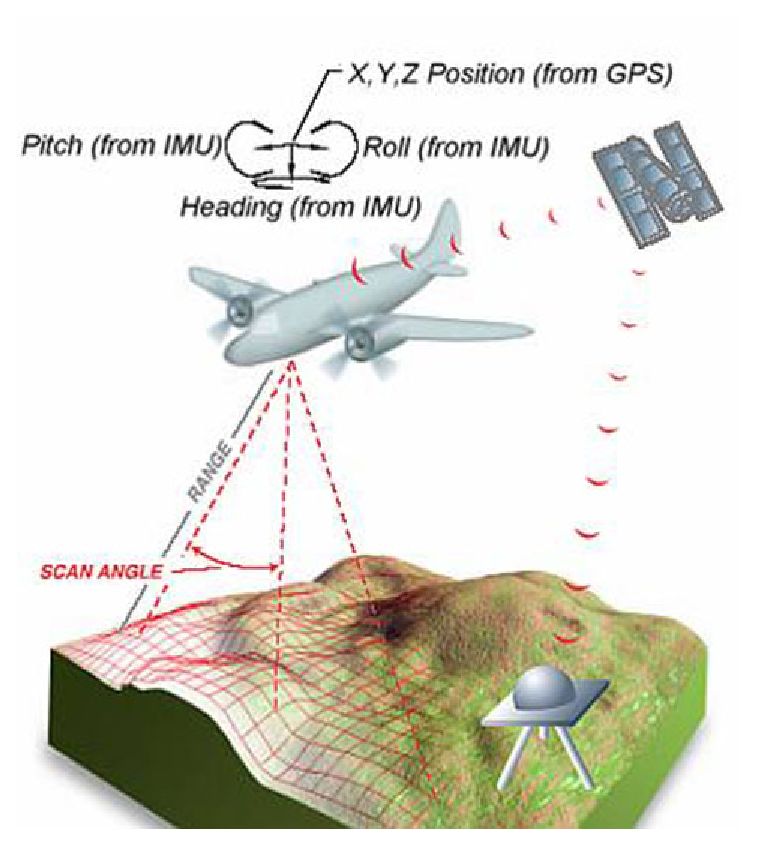
\epsfig{file=images/lidarPlane.eps, scale=0.6}}} \quad
      \subfigure[]{\fbox{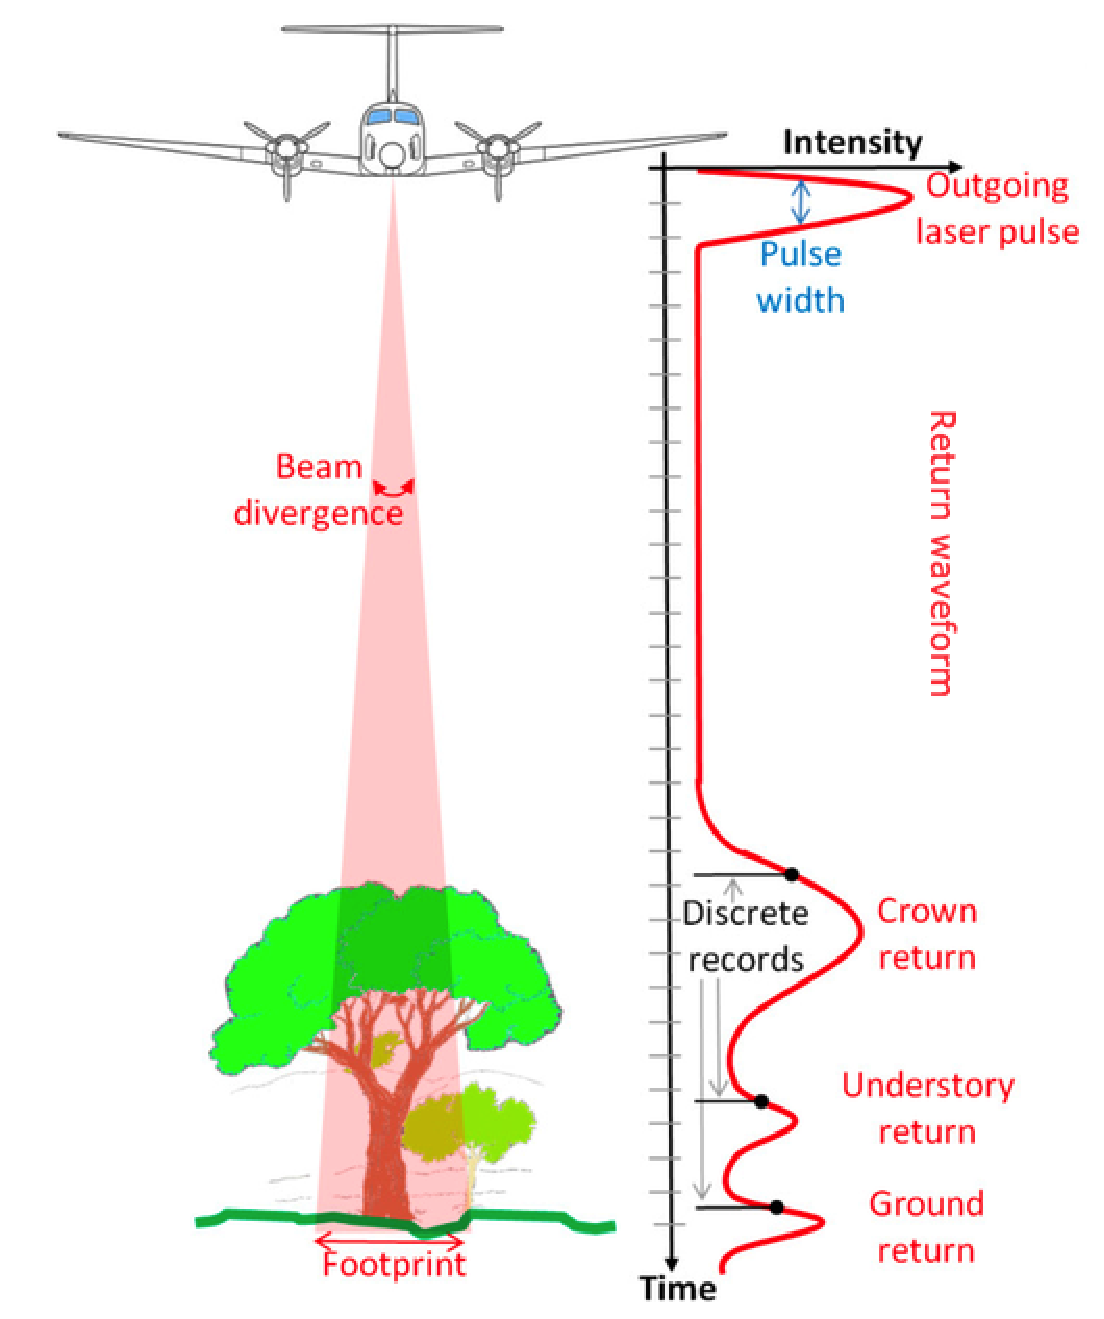
\epsfig{file=images/lidarMultipleReturns.eps, scale=0.38}}} \quad
     }
    
    \caption[Schematic view of a LiDAR flight]{A) Schematic view of a LiDAR flight: GPS coordinates, IMU coordinates, and tilt angle of pulse together determine the position of the point on the ground (Source: Ohio Department of Transportation). B) Return waveform of a single LiDAR pulse both in its actual continuous form and its 3 discrete records (crown, understory, and ground) each as a point in the point cloud \citep{fernandez2014now}.}
    \label{fig:lidar}
  \end{center}
\end{figure}





%\begin{figure}[b!]
%  \centering
%    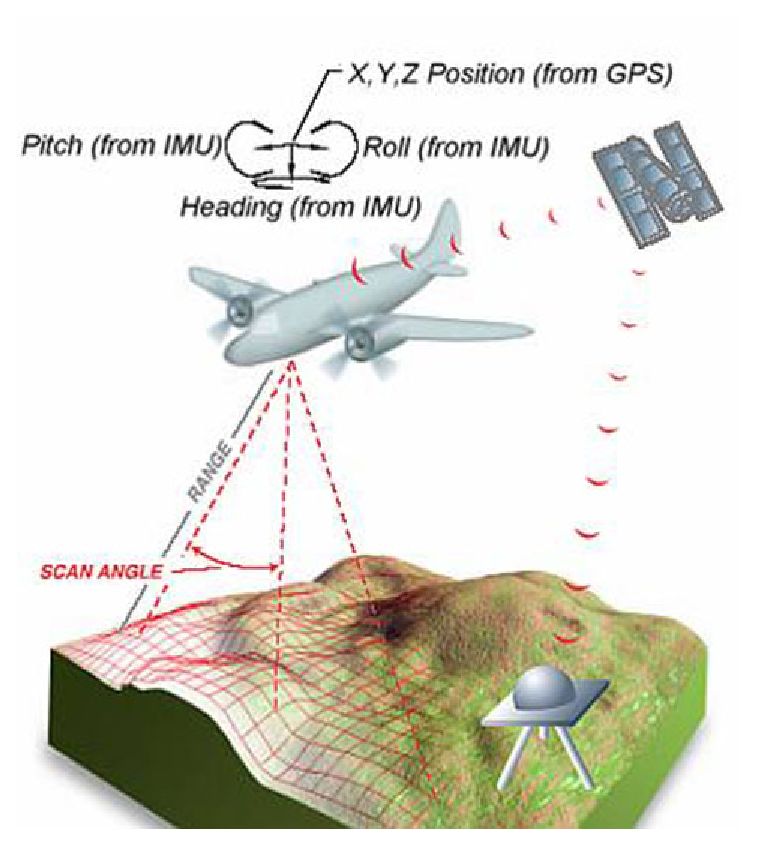
\includegraphics[scale=0.45]{images/lidarPlane.eps}
%    \caption[Schematic view of a LiDAR flight]{Schematic view of a LiDAR flight: GPS coordinates, IMU coordinates, and tilt angle of pulse together determine the position of the point on the ground (Source: Ohio Department of Transportation).}
%    \label{fig:lidar plane}
%\end{figure}

Each LiDAR pulse can have multiple returns depending if it can penetrate through and how much signal intensity is reflected back. Figure~\ref{fig:lidar} (B) shows how each LiDAR pulse can have multiple return values.

%\begin{figure}[b!]
%  \centering
%    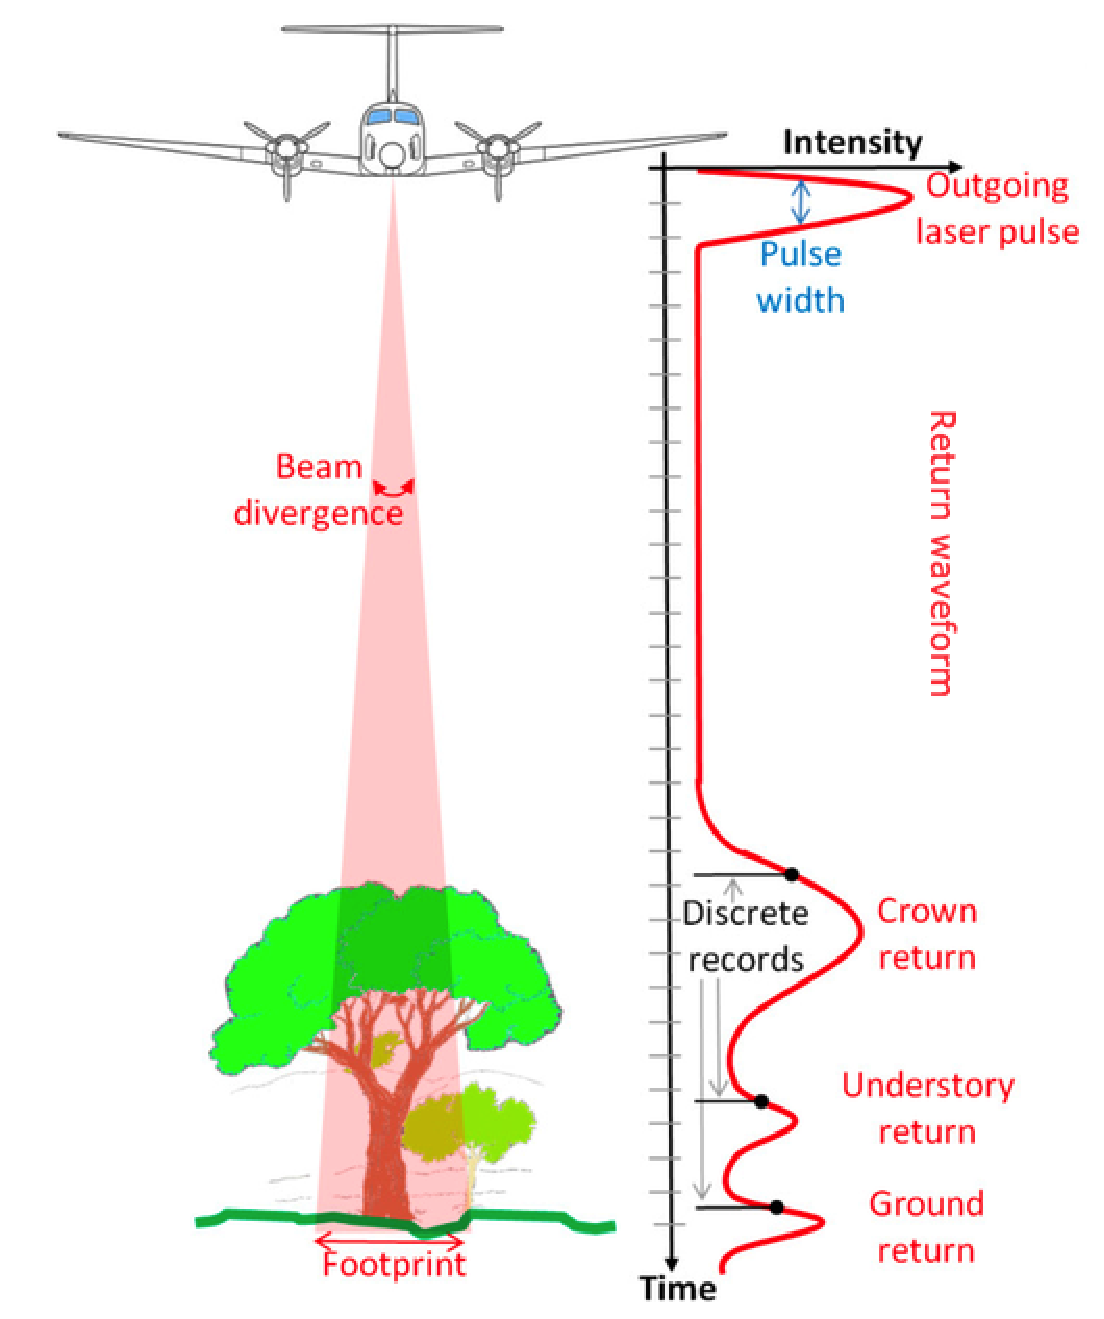
\includegraphics[scale=0.30]{images/lidarMultipleReturns.eps}
%    \caption[Multiple returns of a LiDAR pulse]{Multiple returns of a LiDAR pulse \citep{fernandez2014now}.}
%    \label{fig:lidar multiple returns}
%\end{figure}

Unlike hyperspectral imaging, LiDAR returns a long list of points <x (latitude), y (longtitude), z (elevation), i (intensity), n (number of this return for given pulse), d (direction of scan), e (edge of flight line), t (time)>



For lidar usually green or near infrared is used as it has high reflectance from vegetation.





%
%
%\begin{figure}
%        \centering
%        \begin{subfigure}[b]{0.3\textwidth}
%                \includegraphics[width=\textwidth]{images/lidarPlane.eps, scale=0.6}
%                \caption{A gull}
%                \label{fig:gull}
%        \end{subfigure}%
%        ~ %add desired spacing between images, e. g. ~, \quad, \qquad, \hfill etc.
%          %(or a blank line to force the subfigure onto a new line)
%        \begin{subfigure}[b]{0.3\textwidth}
%                \includegraphics[width=\textwidth]{tiger}
%                \caption{A tiger}
%                \label{fig:tiger}
%        \end{subfigure}
%        ~ %add desired spacing between images, e. g. ~, \quad, \qquad, \hfill etc.
%          %(or a blank line to force the subfigure onto a new line)
%        \begin{subfigure}[b]{0.3\textwidth}
%                \includegraphics[width=\textwidth]{mouse}
%                \caption{A mouse}
%                \label{fig:mouse}
%        \end{subfigure}
%        \caption{Pictures of animals}\label{fig:animals}
%\end{figure}















\section{Data Variety}

As of 


%\begin{table}[h!]
%\caption{How to align decimals in a numerical column}\label{tb1}
%  \begin{tabular}{p{3 in} r@{.}l c}
% \hline
% Category & \multicolumn{2}{c}{Result}  & \hspace{2.2 in} \\
% \hline
%  first & 3&14159 & \hspace{2.2 in} \\
%  second & 16&2 & \hspace{2.2 in} \\
%  third & 123&456 & \hspace{2.2 in} \\
%  \hline
%  \end{tabular}
%\end{table}
%
%
%\begin{figure}[htbp]
%  \centering
%    \includegraphics[width=3in, scale=0.5]{images/LaTeX2e_logo.eps}
%    \caption[\LaTeX 2\ensuremath{\epsilon} logo(resized for no reason)]{\LaTeX 2\ensuremath{\epsilon} logo, resized for no reason. This caption is being extended in order to test that it has the correct indentation.}
%\end{figure}





%
%\begin{figure}[htbp]
%  \begin{center}
%    \centering
%    \mbox{
%      \subfigure[]{\epsfig{file=images/mouse.eps, scale=0.6}} \quad
%      \subfigure[]{\begin{turn}{20}\epsfig{file=images/mouse.eps, scale=0.6}\end{turn}} \quad
%     }
%    \mbox{
%      \subfigure[]{\begin{turn}{-20}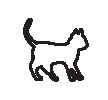
\epsfig{file=images/cat.eps, scale=3}\end{turn}} \quad
%      \subfigure[]{\begin{turn}{-10}\epsfig{file=images/mouse.eps, scale=0.6}\end{turn}} \quad
%      }
%    \caption[Tom and Jerry]{Tom and Jerries? A) Mouse 1 B) mouse 2 C) Hungry Cat D) mouse 3}
%    \label{mice}
%  \end{center}
%\end{figure}

\subsection{Markov Logic Network}
Markov logic network is a probabilistic logic that applies the concept of Markov network to first order logic. For inference, instead of usning intractable algorithms of prolog or lisp, it uses MCMC sampling.

\section{Proposed Work}

\section{Proposal Structure}

% Mapping the spatial distribution of plant species in savannas provides insight into the roles of competition, fire, herbivory, soils and climate in maintaining the biodiversity of these ecosystems. 
 
% Savannas harbor spatially complex assemblages of vegetation that are mediated by an array of biotic and abiotic factors including plant competition, fire, herbivory, soils and climate [1–4]. Mapping the distribution of species abundances across spatial scales relevant to these processes is requisite to understanding their role in shaping and maintaining savanna biodiversity.
 
%%% Invasive plant species can change entire habitats by penetrating the native canopy and eventually replacing it [1]. At times, fundamental ecosystem processes such as nitrogen (N) cycling as well as disturbance regimes such as fire frequency are altered by the introduced species, resulting in a major change in biological diversity and ecosystem functioning [2].
 
% Effective management of introduced species starts with monitoring and mapping, which is a central component of the biological diversity protection programs of many government agencies and non- governmental organizations worldwide [3]. Remote detection and mapping of biodiversity and invasive species from airborne or spaceborne instruments is promising (review by [4]), but operational approaches are lacking because of our limited biophysical understanding of when remotely sensed signatures indicate the presence of unique species—native or invasive—within and across ecosystems. The spectra express the biochemical and structural properties of the vegetation, but translating that to species composition requires an increased understanding of the """""""spectral separability""""""""" of species at different levels of ecological and taxonomic aggregation.
 
 
%%%% Tropical forests store a large proportion of terrestrial carbon. For example, Dixon et al. (1994) estimated that low-latitude tropical forests contain 59\% and 27\% of carbon stored in global forest vegetation and soil pools, respectively. There still remains considerable uncertainty in global and regional estimates of carbon stocks and dynamics. 

\chapter{Species Classification}
\label{chapter:Species Classification}

\section{Species Classification using SVM}

SVM paper

\section{Unmixing: MESMA, SPICE, PCOMMEND}

MESMA results and overview SPICE, PCOMMEND

\section{LiDAR Stack and Field Statistics}

watershed

\chapter{Information Extraction from Text}
\label{chapter:Information Extraction from Text}

TREC KBA paper
\chapter{QUANTUM CHEMISTRY}%
\label{ch_QC}

I've borrowed a few examples of equations I've run across to illustrate how the equations should look in the thesis or dissertation. \cite{Agarwal06}

\section{The Electronic Problem}

The starting point of any discussion of quantum mechanics is the non-relativistic, time-dependent Shr\"{o}dinger equation~\cite{Sza89},

\begin{gather}
{\it i}\hbar\frac{\partial}{\partial t}\Psi(r,t)=\hat{H}\Psi(r,t)\hspace{0.2cm},
\end{gather}

\noindent where $\hbar$ is Planck's constant, $\Psi(r,t)$ is the wave function of the quantum system and $\hat{H}$ is the Hamiltonian, which is an operator that contains a kinetic energy term and a potential energy term.

When we restrict the wave function to be a product of a function of time and a function of space, as, for example, is the case when the potential energy term of the Hamiltonian is independent of time, the time-independent Scrh\"{o}dinger equation can be expressed as:

\begin{gather}
\hat{H}\Psi=E\Psi\hspace{0.2cm}.
\end{gather}

The specific form of the Hamiltonian for molecules is:

\begin{gather}
\label{molH}
{\begin{split}
\hat{H} =-\sum_{A=1}^{M} \frac{1}{2M_{A}} \nabla^{2}_{A} - \sum_{i=1}^{N} \frac{1}{2} \nabla^{2}_{i} - \sum_{i=1}^{N}\sum_{A=1}^{M}\frac{Z_{A}}{r_{iA}} \\
 + \sum_{i=1}^{N}\sum_{j>i}^{N} \frac{1}{r_{ij}} + \sum_{A=1}^{M}\sum_{B>A}^{M} \frac{Z_{A} Z_{B}}{R_{A B}}\hspace{0.2cm},
\end{split}}
\end{gather}

\noindent where $A$ and $B$, etc., label nuclei, and {\it i}, {\it j}, etc., label electrons, $Z$ is the atomic number, and Hartree atomic units ($\hbar = e= m_e = 1$) have been used.


The Born-Oppenheimer approximation, which is a useful and central approximation in quantum chemistry, separates electronic and nuclear motions. Assuming that the nuclei are fixed (since nuclei are much heavier than the electrons), the nuclear kinetic energy term, which is the first term in equation \eqref{molH}, can be neglected, and the repulsion between nuclei, the third term of equation \eqref{molH}, is a constant. This approximation leads to an electronic Hamiltonian,

\begin{gather}
\label{elecH}
\hat{H}_{elec}=- \sum_{i=1}^{N} \frac{1}{2} \nabla^{2}_{i} - \sum_{i=1}^{N}\sum_{A=1}^{M}\frac{Z_{A}}{r_{iA}} + \sum_{i=1}^{N}\sum_{j>i}^{N} \frac{1}{r_{ij}}\hspace{0.2cm},
\end{gather}

\noindent and the Schr\"{o}dinger equation becomes:

\begin{gather}
\hat{H}_{elec}\Psi_{elec}=E_{elec}\Psi_{elec}\hspace{0.2cm}.
\end{gather}

\section{Hartree-Fock Approximation}

Except for the simple case of $H_2^+$, molecules are many-electron problems and determining accurate molecular orbitals, which are the eigenfunctions of the Schr\"{o}dinger equation for a molecule, has been the main task of quantum chemists for many years. Approximate methods have been developed to solve the Schr\"{o}dinger equation, since it is intractable computationally to find the exact solution for a many-electron system. One approximate method that is used frequently to solve the Schr\"{o}dinger equation is based on Hartree-Fock theory. In the present work, Hartree-Fock is not the main method used, but it is crucial to introduce it to explain the methods on which this work is based.

Consider a trial function in the form of a single N-electron Slater-determinant, which obeys the Pauli exclusion principle,

\begin{gather}
\mid \Psi \rangle = \hat{O}\hat{A}\mid \phi_1\phi_2 ...\phi_{\alpha}... \phi_N\rangle\hspace{0.2cm}.
\end{gather}

Here $\hat{O}$ is the spin projector operator that ensures that the wave function remains an eigenfunction of the spin-squared operator ($\hat{S}^2$), $\hat{A}$ is the antisymmetrizer, $\phi_{\alpha}$ is a one-electron wave function that represents the molecular orbital, and Dirac notation has been adopted.

The molecular orbitals can be expanded as a linear combination of atomic orbitals $\psi_{\alpha}$ ,

\begin{gather}
\phi_i=\sum_u\chi_uC_{ui}=XC_i\hspace{0.2cm},
\end{gather}

\noindent which constitute the basis set for the calculation.

$\Psi$ is varied with respect to $C$ following the variational principle to minimize the expectation value of the electronic Hamiltonian, $\hat{H}$ (where the electronic subscript has been dropped for simplicity) to give the following expression for the effective one-particle Fock operator, $f$,

\begin{gather}
f\mid\phi_i\rangle=[h+\sum_{j=1}^{N}J_{j}-K_{j}]\mid\phi_i\rangle=\sum_{j=1}^{N}\epsilon_{ji}\mid\phi_j\rangle\hspace{0.2cm},
\end{gather}

\noindent where $h$ represents the first two terms of equation \eqref{elecH} and $J$ and $K$ are the coulomb and exchange operators respectively. Using a unitary basis to diagonalize the Hermitian matrix, $\epsilon$, with matrix elements $\epsilon_{ji}$ yields the canonical Hartree-Fock equation,

\begin{gather}
f\phi_i=\epsilon_i\phi_i\hspace{0.2cm}.
\end{gather}

From this equation the following generalized-eigenvalue expression can be obtained,

\begin{gather}
FC=SCE\hspace{0.2cm},
\end{gather}

\noindent where $F$ is the Fock matrix, $C$ is a square matrix containing the molecular orbital coefficients, $S$ is the overlap matrix and $E$ is the energy matrix containing the orbital energies $\epsilon_i$.

The Fock matrix elements are,

\begin{gather}
{\begin{split}
F_{uv}=\langle\chi_u \mid f \mid \chi_v \rangle = \langle u \mid f \mid v \rangle \\
= H_{uv}+ \sum_{s,t} P_{st}[\langle us \mid vt \rangle - \frac{ \langle us \mid tv \rangle}{2} ]\hspace{0.2cm},
\end{split}}
\end{gather}

$P$ is the density matrix,

\begin{gather}
P_{uv}=\sum_{a}C_{ua}C_{va}n_a\hspace{0.2cm},
\end{gather}

\noindent where $n_a$ is the occupation number.

The overlap matrix elements are,

\begin{gather}
S_{uv}=\langle\chi_u\mid\chi_v\rangle=\langle u \mid  v \rangle\hspace{0.2cm}.
\end{gather}

A self-consistent solution of the previous equations is known as the Hartree-Fock, Self-Consistent Field (SCF) methodology.

These {\it ab initio} expressions for the Fock matrix will be used below to explain additional details of the methods used in this research.


\chapter{MATH, FIGURES, AND TABLES}
\section{Text Flow: Problems and Solutions}
Let's face it. LaTeX is used because you can type very complicated formulas and equations without ever touching a mouse! And in most situations, where the spacing requirements are not as demanding as the UF Theses and Dissertation requirements, LaTeX's  love of white space would not pose a problem.

%\begin{algorithm}
%\caption{Euclid�s algorithm}\label{euclid}
%\begin{algorithmic}[1]
%\Procedure{Euclid}{$a,b$}\Comment{The g.c.d. of a and b}
%\State $r\gets a\bmod b$
%\While{$r\not=0$}\Comment{We have the answer if r is 0}
%\State $a\gets b$
%\State $b\gets r$
%\State $r\gets a\bmod b$
%\EndWhile\label{euclidendwhile}
%\State \textbf{return} $b$\Comment{The gcd is b}
%\EndProcedure
%\end{algorithmic}
%\end{algorithm}

However, you ARE producing this document for the UF Graduate School and their spacing requirements ARE quite demanding. Pages, other than the last page of a chapter, are supposed to be full. LaTeX has a tendency to break a page early rather than split a display element (equation array, align, theorem, table, figure, etc.). To help in this matter there are three lines in the preamble of the ufsampleETD.tex file. These are:
\begin{verbatim}
\renewcommand{\topfraction}{0.85}
\renewcommand{\textfraction}{0.1}
\renewcommand{\floatpagefraction}{0.75}
\end{verbatim}

However, even with these commands LaTeX likes to break pages rather than equation arrays, theorems, postulates, proofs, etc. If you find that these elements are causing pages to break badly you can un-comment the command \verb=\allowdisplaybreaks= and with any luck, that will cure the problem. If not, it may be necessary to break the displays manually which is always the last resort and only done just before final submission.
\section{Equation Notes}
Again, one of the major reasons for using LaTeX in the first place is how it handles the mathematics displays. However, there are a few details you need to be aware of:
\begin{itemize}

    \item If you place an extra carriage return before or after an equation LaTeX will place some extra ``paragraph'' spacing around the equation. Try to avoid this.
    \item If you want to explain your notation in the equation with a list of statements such as; ``where $Z = \gamma$,'' do so in paragraph form rather than a vertical list.
    \item  While every equation does not have to be labeled, determining which items should and should not be labeled can get tricky. Since LaTeX generates the labels automatically it's usually best to let it label as it sees fit. In equation arrays that leads to a final result it's certainly acceptable to suppress the labels on preliminary steps by using the \verb+\nonumber+ command as long as the last line of the procedure has a label.

\end{itemize}

\section{Tables, Figures, and Subfigures}

\subsection{Tables}

Typically, the standard LaTeX table environment is used. Table captions need to be \underline{above} the table, and typically there should not be any vertical lines in the table. Formatting tables in a landscape page is explained in section ~\ref{landscape}.

\begin{table}[htbp]
    \caption{A sample Table}\label{first}
    \begin{tabularx}{6.5in}{XXX}
      \hline
      First & Second & Third \\
      \hline
      12 & 45 & 26 \\
      17 & 32 & 93 \\
      text & 51 & can be there too. \\	
      \epsfig{figure=images/cat.eps, scale=1} & 28 & Figures too - a cat. \\
      \begin{turn}{0}\epsfig{figure=images/mouse.eps, scale=0.25}\end{turn} & 000 & and a mouse! \\
      \hline
    \end{tabularx}
\end{table}


\subsection{Figures}
You can either use \texttt{$\backslash$includegraphics} or {$\backslash$epsfig} commands to include your figures. The appropriate packages are included in the packages.tex file. For additional precaution, a copy of \texttt{rotating.sty} is included in the template. Please do not delete this file. Note that the caption for the figures is \underline{below} the figure. The figures in the table above was inserted with $\backslash$epsfig. Below is a sample file with \texttt{$\backslash$includegraphics}:

\begin{figure}[htbp]
  \centering
    \includegraphics[width=3in, scale=0.5]{images/LaTeX2e_logo.eps}
    \caption[\LaTeX 2\ensuremath{\epsilon} logo(resized for no reason)]{\LaTeX 2\ensuremath{\epsilon} logo, resized for no reason. This caption is being extended in order to test that it has the correct indentation.}
\end{figure}

\subsection{Subfigures}

In addition to the standard \LaTeX options for scaling and rotation, the \texttt{rotating} package has additional options for turning and rotating both text and figures/tables. Please look at the documentation of this package for further details.

For subfigures, please use \red{\texttt{subfigure}} command (see \url{chapter4.tex} for code). We have
made some slight modifications to the subfigure.sty file to match the Editorial Office specification so make sure it is in the same folder as the ufsampleETD.tex file when you compile your document.

\begin{figure}[htbp]
  \begin{center}
    \centering
    \mbox{
      \subfigure[]{\epsfig{file=images/mouse.eps, scale=0.6}} \quad
      \subfigure[]{\begin{turn}{20}\epsfig{file=images/mouse.eps, scale=0.6}\end{turn}} \quad
     }
    \mbox{
      \subfigure[]{\begin{turn}{-20}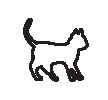
\epsfig{file=images/cat.eps, scale=3}\end{turn}} \quad
      \subfigure[]{\begin{turn}{-10}\epsfig{file=images/mouse.eps, scale=0.6}\end{turn}} \quad
      }
    \caption[Tom and Jerry]{Tom and Jerries? A) Mouse 1 B) mouse 2 C) Hungry Cat D) mouse 3}
    \label{mice}
  \end{center}
\end{figure}

There is some fancy formatting possible with \texttt{subfigure}. For instance, it is possible (but not suggested) to list the captions of each subfigure in the List of Figures in the table of contents. Please look at the documentation of \texttt{subfigure} package for details.


\section{Formatting in Landscape Mode}\label{landscape}

There are many ways to format figures and tables in a landscape. Depending on what you want to use, you can use one of the following enviroments:

\begin{itemize}
\singlespacing
\item The \texttt{landscape} environment \vspace{-12pt}
\item The \texttt{sidewaysfigure} environment \vspace{-12pt}
\item The \texttt{sidewaystable} environment
\end{itemize}
\doublespacing

%%%  \addtocontents{toc}{\protect\pagebreak}% This command starts a new page in the TOC
%%%%%%%%%%%% it allowa you to force a subheading to the next page if necessary

\subsection{The \texttt{landscape} environment}
The \texttt{landscape} environment starts by default a new page, because it changes the two lengths $\backslash$paperwidth and $\backslash$paperheight. Typically you will use the {\texttt{landscape} if you want to have an \underline{\textbf{entire} section or a subsection} in landscape mode (i.e. both text and figures/tables). This should not be used for a just single figure or a table (Use \blue{\texttt{sidewaysfigure}} and  \blue{\texttt{sidewaystable}} described in sub-section \ref{side} instead). In the chapter4.tex file we demonstrate how to force a page break in the Table of Contents. Something that often needs to be done but is not documented in most LaTeX tutorials.

The following sub-subsection is included in an environment like:

\singlespacing
\begin{verbatim}
\begin{landscape}
\subsubsection{Sample Landscape Page}\label{ps}
Note that even though we are in landscape mode,
only the text part is in landscape.
The header and footer (for example the page number) are still
in portrait mode. This $\backslash$begin$\{$landscape$\}$
environment is part of the lscape package. Look at the documentation
of this package for further details and options.
\end{landscape}
\end{verbatim}
\doublespacing

The $\backslash$begin$\{$landscape$\}$ immediately starts the new page, a lot of vertical whitespace, like the one on this page, maybe possible.

The subsubsection command also represents a common error in dissertation/thesis construction. There is only one heading at that level. Whenever a section is divided, it must be divided into two segments - otherwise there is no reason to introduce another category.

\begin{landscape}
\subsubsection{Sample Landscape Page}\label{ps}
It's Important to remember that no headings or paragraph text should actually be on a landscaped page. Only the Figure or Table and their captions. In addition, the landscaped page should be rotated in the pdf so the text on the landscaped page is readable without turning your head sideways. Note that even though we are in landscape mode, only the text part is in landscape, the header and footer (that implement, for example the page number) are still in portrait mode. This  \texttt{landscape} environment is part of the  \texttt{lscape} package. Look at the documentation of this package for more details and options.
\end{landscape}


\subsection{\texttt{sidewaysfigure} and \texttt{sidewaystable} Environments}
\label{side}
With large figures and tables with lots of columns, it is sometimes necessary to rotate them to landscape mode. The \texttt{sidewaysfigure} and the \texttt{sidewaystable} environments from the \texttt{rotating} package can be used for this. Sample code for these two environments are give below:

\singlespacing
\noindent \underline{A Landscape Figure}:
\begin{verbatim}
\begin{sidewaysfigure}
\centerline{\epsfig{figure=images/figurename.eps, scale=0.5}}
\caption{Your Caption for the figue}
\end{sidewaysfigure}

Note: Change value of scale to change your figure size.
      1 is 100%, i.e. original size. You can go beyond 1
      if your file is in a scalable vector graphics format
      like .eps
\end{verbatim}
\doublespacing

\singlespacing
\noindent \underline{A Landscape Table}:
\begin{verbatim}
\begin{sidewaystable}
\centering %optional
\begin{tabular}{rl}
\end{tabular}
\caption{Your Caption for the table}
\end{sidewaystable}
\end{verbatim}
\doublespacing

The above code will produce a figure/table rotated by 90$^\circ$ in the counter-clockwise direction, and will also rotate the caption accordingly as per the Editorial Office requirements. Both these environments are ``intelligent'' in the sense that they will put your figure/table in a new landscape page and will \textbf{NOT} leave empty whitespace before the figure like the \texttt{landscape} environment. The following 'Lorem Ipsum' paragraphs demonstrate this.

% Example of a landscape page setup, this command along with the lscape package effectively rotates all the input
% the tags 90 degrees CCW, but keeps the page orientation

\begin{sidewaysfigure}
\centerline{\epsfig{figure=images/theworld.eps, scale=0.75}} %change value of scale (between 0 to 1) to change your figure size. 1 is 100%, ie original size.
\caption[A landscape figure]{You can turn the world on its heels.}
\end{sidewaysfigure}

Lorem ipsum dolor sit amet, consectetuer adipiscing elit. Integer
ante. Ut tincidunt ultrices turpis. Phasellus nonummy pulvinar sem.
Donec sem nisl, rhoncus eu, porttitor in, blandit nec, arcu.
Vestibulum tincidunt ante. Pellentesque quis massa. Proin vehicula
feugiat turpis. Aenean at tellus sed justo ornare dictum. Nullam sit
amet libero nec lorem sodales cursus. Donec tortor nulla, convallis
in, suscipit in, posuere at, nunc.

Aliquam tortor risus, ultricies sed, eleifend in, congue quis,
justo. Pellentesque egestas orci non urna. Phasellus ligula. Ut
nonummy. Suspendisse potenti. Donec posuere justo quis eros. In
erat. Nunc aliquam metus sed dui. Fusce justo felis, posuere a,
elementum non, semper eget, mi. Morbi iaculis lorem at sem.
Vestibulum ante ipsum primis in faucibus orci luctus et ultrices
posuere cubilia Curae; Cum sociis natoque penatibus et magnis dis
parturient montes, nascetur ridiculus mus. Phasellus velit. Maecenas
libero tortor, pharetra id, dictum ac, lacinia vestibulum, urna.
Lorem ipsum dolor sit amet, consectetuer adipiscing elit. In libero
nunc, fringilla a, condimentum lobortis, consequat eget, quam.
Phasellus eget nisi. Maecenas risus ligula, euismod a, tristique
non, sagittis eu, quam. Donec metus nunc, varius ut, lacinia sit
amet, pellentesque ac, mauris. Nulla mollis aliquam metus.

\begin{sidewaystable}
\centering
    \caption{The Same Table as ~\ref{first}, but in landscape mode}\label{second}
    \begin{tabular}{rl}
      \hline
      First & Second \\
      \hline
      12 & 26 \\
      17 & 93 \\
      text & can be there too. \\	
      \epsfig{figure=images/cat.eps, scale=1} & Figures too - a cat. \\
      \begin{turn}{0}\epsfig{figure=images/mouse.eps, scale=0.25}\end{turn} & and a mouse! \\
      \hline
    \end{tabular}
\end{sidewaystable}

Lorem ipsum dolor sit amet, consectetuer adipiscing elit. Integer
ante. Ut tincidunt ultrices turpis. Phasellus nonummy pulvinar sem.
Donec sem nisl, rhoncus eu, porttitor in, blandit nec, arcu.
Vestibulum tincidunt ante. Pellentesque quis massa. Proin vehicula
feugiat turpis. Aenean at tellus sed justo ornare dictum. Nullam sit
amet libero nec lorem sodales cursus. Donec tortor nulla, convallis
in, suscipit in, posuere at, nunc.
%\begin{definition}
%\begin{algorithm}
%  \caption{Counting mismatches between two packed DNA strings
%    \label{alg:packed-dna-hamming}}
%  \begin{algorithmic}[1]
%    \Require{$x$ and $y$ are packed DNA strings of equal length $n$}
%    \Statex
%    \Function{Distance}{$x, y$}
%      \Let{$z$}{$x \oplus y$} \Comment{$\oplus$: bitwise exclusive-or}
%      \Let{$\delta$}{$0$}
%      \For{$i \gets 1 \textrm{ to } n$}
%        \If{$z_i \neq 0$}
%          \Let{$\delta$}{$\delta + 1$}
%        \EndIf
%      \EndFor
%      \State \Return{$\delta$}
%    \EndFunction
%  \end{algorithmic}
%\end{algorithm}
%\end{definition}
Aliquam tortor risus, ultricies sed, eleifend in, congue quis,
justo. Pellentesque egestas orci non urna. Phasellus ligula. Ut
nonummy. Suspendisse potenti. Donec posuere justo quis eros. In
erat. Nunc aliquam metus sed dui. Fusce justo felis, posuere a,
elementum non, semper eget, mi. Morbi iaculis lorem at sem.
Vestibulum ante ipsum primis in faucibus orci luctus et ultrices
posuere cubilia Curae; Cum sociis natoque penatibus et magnis dis
parturient montes, nascetur ridiculus mus. Phasellus velit. Maecenas
libero tortor, pharetra id, dictum ac, lacinia vestibulum, urna.
Lorem ipsum dolor sit amet, consectetuer adipiscing elit. In libero
nunc, fringilla a, condimentum lobortis, consequat eget, quam.
Phasellus eget nisi. Maecenas risus ligula, euismod a, tristique
non, sagittis eu, quam. Donec metus nunc, varius ut, lacinia sit
amet, pellentesque ac, mauris. Nulla mollis aliquam metus.


\section{Some bugs and fixes}

A quirk in the \LaTeX 2\ensuremath{\epsilon} template is
the centering of table and figure captions \ldots which the editorial
office will not accept. This is actually only a problem for captions
that are less than the width of the paper(within the margins that
is). A fix has already been implemented in the template for this issue.

However, if you find your short captions are
being centered in spite of the new caption package options, try
using the following codes, which each differ ever so slightly
depending if the caption is for a table or figure. Inserting the
given code in the table or figure environments just after you
declare the start of that environment for each table or $\backslash$landscape environment figure that
has a short caption that is being centered:

\singlespacing%
\noindent \underline{For Tables}:

\begin{verbatim}
  \makeatletter
\long\def\@makecaption#1#2{%
  \vskip\abovecaptionskip
  \sbox\@tempboxa{#1: #2}%
  \ifdim \wd\@tempboxa >\hsize
    #1: #2\par
  \else
    \global \@minipagefalse
    \hb@xt@\hsize{\box\@tempboxa\hfil}%
  \fi}
\makeatother
\end{verbatim}

\vspace{12pt}

\noindent \underline{For Figures}:
\begin{verbatim}
\makeatletter
\long\def\@makecaption#1#2{%
  \vskip\abovecaptionskip
  \sbox\@tempboxa{#1: #2}%
  \ifdim \wd\@tempboxa >\hsize
    #1: #2\par
  \else
    \global \@minipagefalse
    \hb@xt@\hsize{\box\@tempboxa\hfil}%
  \fi
  \vskip\belowcaptionskip}
\makeatother
\end{verbatim}
\doublespacing






\chapter{Conclusion}
\chapter{CONCLUSION}

%-----------------------------------------------------------------------%

% Use the appropriate file depending upon the number of appendices you have


%% The Editorial Office Requirements for the Table of Contents cause a significant problem 
%in Latex if there is only one Appendix. The Appendix is no longer labeled "A" in the TOC
%but has the word "APPENDIX" placed in front of the title of the Appendix. This can be done
%without issue IF nothing needs to be numbered by LaTeX in the Appendix. Unfortunately, most of the time
%something needs to be numbered in that single Appendix. For this reason we have included the IFTHENELSE switch
%found in this document and at the beginning of AppendixA. We assume that if you have any appendices, that you have more than one. However, you DO only have one appendix DO NOT USE THIS FILE!!!!!!!!!!!!!!!!!!!!!!!
%
% appendix1.tex has all the settings needed to adjust for a single appendix
% you will have a major problem with your TOC if you use this file with a single appendix!!!!!

%
% Comment (or delete) all of the \input{AppendixB} commands except those you are using.
%Then open the AppendixA.tex file and continue there.

%you can add/substract individual appendices through by using the /include{appendix'X'}
% and creating/deleting the appropriate files
\appendix %
%\clearpage%


\addtocontents{toc}{\protect\addvspace{10pt}\protect\noindent \protect APPENDIX}

% % % % % % % If you have a single appendix, you should be using appendix1.tex
% % % % % % % NOT this file

{\chapter{THIS IS THE FIRST APPENDIX}

Lorem ipsum dolor sit amet, consectetuer adipiscing elit. Maecenas
eget magna. Aenean et lorem. Ut dignissim neque at nisi. In hac
habitasse platea dictumst. In porta ornare eros. Nunc eu ante. In
non est vehicula tellus cursus suscipit. Proin sed libero. Sed risus
enim, eleifend in, pellentesque ac, nonummy quis, nulla. Phasellus
imperdiet libero nec massa. Ut sapien libero, adipiscing eu,
volutpat porttitor, ultricies eget, nisi. Sed odio. Suspendisse
potenti. Duis dolor augue, viverra id, porta in, dignissim id, nisl.
Vivamus blandit cursus eros. Maecenas sit amet urna sit amet orci
nonummy pharetra.

Praesent cursus nibh et mauris. In aliquam felis sit amet ligula.
Nulla faucibus nisl eget nisl. Aliquam tincidunt. Mauris eget elit
sed massa luctus posuere. Pellentesque suscipit. In odio urna,
semper ut, convallis ut, porta et, nibh. Nulla sodales metus nec
velit posuere gravida. Cras tristique. Etiam urna risus, accumsan
ut, placerat sed, iaculis id, est.

Nullam mi. Pellentesque habitant morbi tristique senectus et netus
et malesuada fames ac turpis egestas. Duis vitae metus in massa
hendrerit rhoncus. Fusce tortor justo, laoreet eu, facilisis at,
gravida et, felis. Donec imperdiet mollis erat. Integer tempus nulla
ac lorem. Fusce porttitor. Aenean quis arcu. Morbi consectetuer, leo
eu mollis elementum, urna massa malesuada risus, euismod tempor
lorem elit ut mauris. Cras elit orci, facilisis ac, mattis iaculis,
cursus ac, augue. Donec eget nisl. Pellentesque fermentum sodales
nibh. Vivamus non risus. Donec est libero, tincidunt sit amet,
pretium vitae, blandit sed, tellus. Nunc diam risus, interdum sed,
laoreet quis, varius ac, turpis. In et purus eget nibh vehicula
rhoncus. Aenean et neque. Praesent nisl nisi, tempus quis, nonummy
ac, auctor a, neque. Suspendisse et metus. Suspendisse non metus eu
mauris auctor sagittis.
 %
\chapter{AN EXAMPLE OF A HALF TITLE PAGE}%
\label{appendixB}

\clearpage %remove this command if your appendix doesn't start with a landscaped page!!!!!
\thispagestyle{plain}
\begin{landscape}
\begin{figure}

  \begin{center}
    \includegraphics[width=6in]{images/LaTeX2e_logo.eps}
    \caption{\LaTeX 2\ensuremath{\epsilon.} logo}\label{biglogo}
  \end{center}
\end{figure}
\end{landscape}


This is how a section should look if the first page is a landscape page.
Lorem ipsum dolor sit amet, consectetuer adipiscing elit. Ut sit
amet nulla. Integer mauris turpis, dapibus ac, auctor non, vehicula
sit amet, magna. Suspendisse eu tellus. Etiam porta. Donec magna.
Donec ut dui. In hac habitasse platea dictumst. Nullam suscipit, mi
at adipiscing commodo, lorem erat scelerisque erat, non pulvinar leo
mi eu metus. Phasellus id felis. Sed quam purus, molestie quis,
ultrices nec, dictum at, magna. Proin viverra viverra ante.

Maecenas sagittis magna quis ligula. Duis vestibulum mi a felis.
Aenean accumsan mattis massa. Nullam lacus sem, consectetuer non,
condimentum sit amet, pharetra ac, odio. Morbi nisi magna, tincidunt
sed, placerat nec, tincidunt id, lectus. Donec ac dui non mauris
vulputate aliquam. Nullam scelerisque congue pede. Integer ipsum.
Vestibulum auctor. Suspendisse eget leo id libero cursus dictum. Sed
malesuada. Aliquam imperdiet. Donec dui metus, porta eu, aliquet
vel, vulputate vitae, lacus.

Nulla quis purus id turpis luctus feugiat. Fusce feugiat. Proin
felis. Morbi elit est, fermentum in, tincidunt vitae, convallis vel,
orci. Vestibulum justo. Suspendisse non nisl. Pellentesque pretium
adipiscing elit. Phasellus fermentum consequat augue. Sed pede nisl,
fermentum vel, vulputate id, sollicitudin sed, ligula. Cras
suscipit, quam et euismod sagittis, nisl felis gravida felis, quis
pulvinar purus est vel pede. Suspendisse mattis est ac nunc.
Curabitur rutrum, turpis sit amet commodo tempus, metus lorem
commodo lectus, eget fringilla justo nisi et purus. Ut quam sapien,
vehicula quis, rhoncus non, sagittis nec, risus.

Donec eget augue ac lacus adipiscing porta. Maecenas pede. Vivamus
molestie. Duis condimentum ligula auctor pede. Nullam ullamcorper
rhoncus erat. Ut ornare interdum urna. Suspendisse potenti.
Curabitur mattis mauris nec risus. Aenean iaculis turpis eu tortor.
Donec nec ante non mauris pellentesque fringilla.

Phasellus vitae dui id orci sodales cursus. Curabitur sed nulla quis
mauris tincidunt iaculis. Vivamus semper semper orci. Phasellus
suscipit ante vitae leo. Sed arcu ipsum, condimentum id, luctus in,
sodales eu, magna. In dictum, arcu quis pharetra vestibulum, ante
enim placerat lacus, vitae placerat est leo vitae elit. Pellentesque
bibendum enim vulputate eros. Nunc laoreet. Pellentesque habitant
morbi tristique senectus et netus et malesuada fames ac turpis
egestas. Praesent purus odio, euismod sit amet, aliquam a, volutpat
in, augue. Phasellus id massa. Suspendisse suscipit ligula pharetra
dolor. Pellentesque vel pede.

Aliquam pharetra est sit amet magna. Aliquam varius. Donec eu lectus
et nisl iaculis porttitor. Morbi mattis, mauris sed luctus
hendrerit, nulla velit molestie dolor, ac volutpat urna augue vel
quam. Maecenas pellentesque libero et massa. Integer vestibulum,
lacus at mattis euismod, nisl arcu commodo lectus, ut euismod dolor
ligula sit amet libero. Nam in ligula sit amet ante eleifend
aliquet. Phasellus feugiat erat at nulla. Proin in lectus. Proin
laoreet leo laoreet leo congue lacinia. Quisque non diam sit amet
enim ultrices commodo. Praesent fermentum lectus sed ligula. Integer
pulvinar accumsan pede. Quisque molestie ligula eget odio.
Vestibulum ante ipsum primis in faucibus orci luctus et ultrices
posuere cubilia Curae;
 % 
\chapter{DERIVATION OF THE $\Upsilon$ FUNCTION}%
\label{appendixC}

%\clearpage %remove this command if your appendix doesn't start with a landscaped page!!!!!
%\thispagestyle{plain}
%\begin{landscape}
%\begin{figure}

 % \begin{center}
  %  \includegraphics[width=6in]{LaTeX2e_logo.eps}
   % \caption{\LaTeX 2\ensuremath{\epsilon.} logo}\label{biglogo}
  %\end{center}
%\end{figure}
%\end{landscape}

%%%%%%%%%%%%%%%%%%%%%%%%%%%%%%%%%%%%%%%%%%%%%%%%%%%%%%%%%%%%%%%%%%%%%%%%%%%%%%%%%%%%%%%%%%%%%%%%%%


%ADD LABEL

%%%%%%%%%%%%%%%%%%%%%%%%%%%%%%%%%%%%%%%%%%%%%%%%%%%%%%%%%%%%%%%%%%%%%%%%%%%%%%%%%%%%%%%%%%%%%%%%%%

\proposition{The Upsilon Function}\label{first}

(1) If $\beta>0$ and $\alpha\neq0$, then for all $n\geq-1$,

$$I_{n}(c;\alpha; \beta; \delta) = - \frac{e^{\alpha c}}{\alpha} \sum_{i=0}^{n}(\frac{\beta}{\alpha})^{n-i} Hh_{i}(\beta c -\delta)$$

$$+ (\frac{\beta}{\alpha})^{n+1} \frac{\sqrt{2 \pi}}{\beta} e^{\frac{\alpha \delta}{\beta}+\frac{\alpha^{2}}{2\beta^{2}}} \phi(-\beta c + \delta + \frac{\alpha}{\beta})$$
(2) If $\beta<0$ and $\alpha<0$, then for all $x \geq -1$

$$I_{n}(c;\alpha; \beta; \delta) = - \frac{e^{\alpha c}}{\alpha} \sum_{i=0}^{n}(\frac{\beta}{\alpha})^{n-i} Hh_{i}(\beta c -\delta)$$

$$- (\frac{\beta}{\alpha})^{n+1} \frac{\sqrt{2 \pi}}{\beta} e^{\frac{\alpha \delta}{\beta}+\frac{\alpha^{2}}{2\beta^{2}}} \phi(\beta c - \delta - \frac{\alpha}{\beta})$$

\begin{proof}{Case 1.}

$\beta>0$ and $\alpha\neq0$. Since, for any constant $\alpha$ and $n \geq 0$, $e^{\alpha x} Hh_{n}(\beta x - \delta) \rightarrow 0$ as $x \rightarrow \infty$ thanks to (B4), integration by parts leads to

$$I_{n}=-\frac{1}{\alpha}Hh(\beta c -\delta) e^{\alpha c} + \frac{\beta}{\alpha}\int_{c}^{\infty} e^{\alpha x} Hh_{n-1}(\beta c - \delta)dx$$

In other words, we have a recursion, for $n \geq 0$, $I_{n}=-(e^{\alpha c}{\alpha})Hh_{n}(\beta c - \delta) + (\frac{\beta}{\alpha})I_{n-1}$ with

$$I_{-1}=\sqrt{2 \pi} \int_{c}{\infty}e^{\alpha x}\varphi(-\beta x +\delta)dx$$

$$=\frac{\sqrt{2 \pi}}{\beta} e^{\frac{\alpha \delta}{\beta}+\frac{\alpha^{2}}{2 \beta^{2}}}\phi(-\beta c + \delta +\frac{\alpha}{\beta})$$

Solving it yields, for $n \geq -1$,

$$I_{n}=-\frac{e^{\alpha c}}{\alpha}\sum_{i=0}^{n}(\frac{\beta}{\alpha})^{i}Hh_{n-i}(\beta c+\delta) + (\frac{\beta}{\alpha})^{n+1}I_{-1}$$

$$=-\frac{e^{\alpha c}}{\alpha}\sum_{i=0}^{n}(\frac{\beta}{\alpha})^{n-i} Hh_{i}(\beta c+\delta)$$

$$+ (\frac{\beta}{\alpha})^{n+1}\frac{\sqrt{2 \pi}}{\beta} e^{\frac{\alpha \delta}{\beta}+\frac{\alpha^{2}}{2 \beta^{2}}}\phi(-\beta c + \delta +\frac{\alpha}{\beta})$$

where the sum over an empty set is defined to be zero.
\end{proof}

Case2. $\beta<0$ and $\alpha<0$. In this case, we must also have, for $n \geq 0$ and any constant $\alpha<0, e^{\alpha x}Hh_{n}(\beta x -\delta) \rightarrow 0$ as

$x \rightarrow \infty$, thanks to (B5). Using integration by parts, we again have the same recursion, for $n \geq 0, I_{n}=-(e^{\alpha c}/\alpha)Hh_{n}(\beta c - \delta)+(\beta / \alpha)I_{n-1}$, but with a different initial condition

$$I_{-1}=\sqrt{2 \pi}\int_{c}^{\infty}e^{\alpha x}\varphi(-\beta x + \delta)dx$$

$$=-\frac{\sqrt{2 \pi}}{\beta} exp\{\frac{\alpha \delta}{\beta}+\frac{\alpha^{2}}{2 \beta^{2}}\}\phi(\beta c - \delta -\frac{\alpha}{\beta})$$

Solving it yields (B8), for $n \geq -1$.

Finally, we sum the double exponential and the normal random variables

Proposition B.3.

Suppose $\{\xi_{1},\xi_{2},...\}$ is a sequence of i.i.d. exponential random variables with rate $\eta>0$, and Z is a normal variable with distribution $N(0,\sigma^{2})$. Then for every $ n \geq 1$, we have: (1) The density functions are given by:

$$f_{Z+\sum_{i=1}^{n}\xi_{i}}(t)=(\sigma\eta)^{n}\frac{e^{(\sigma\eta)^{2}/2}}{\sigma\sqrt{2\pi}}e^{-t\eta}Hh_{n-1}(-\frac{t}{\sigma}+\sigma\eta)$$

$$f_{Z-\sum_{i=1}^{n}\xi_{i}}(t)=(\sigma\eta)^{n}\frac{e^{(\sigma\eta)^{2}/2}}{\sigma\sqrt{2\pi}}e^{-t\eta}Hh_{n-1}(\frac{t}{\sigma}+\sigma\eta)$$
(2) The tail probabilities are given by

$$P(Z+\sum_{i=1}^{n}\xi_{i}\geq x) = (\sigma\eta)^{n}\frac{e^{(\sigma\eta)^{2}/2}}{\sigma\sqrt{2\pi}}e^{-t\eta}I_{n-1}(x;-\eta,-\frac{1}{\sigma},-\sigma\eta)$$

$$P(Z-\sum_{i=1}^{n}\xi_{i}\geq x) = (\sigma\eta)^{n}\frac{e^{(\sigma\eta)^{2}/2}}{\sigma\sqrt{2\pi}}e^{-t\eta}I_{n-1}(x;\eta,\frac{1}{\sigma},-\sigma\eta)$$

Proof. Case 1. The densities of $Z+\sum_{i=1}^{n}\xi_{i}$, and $Z-\sum_{i=1}^{n}\xi_{i}$. We have

$$f_{Z+\sum_{i=1}^{n}\xi_{i}}(t)=\int_{-\infty}^{\infty}f_{\sum_{i=1}^{n}\xi_{i}}(t-x)f_{Z}(x)dx$$

$$=e^{-t\eta}(\eta^{n})\int_{-\infty}{t}\frac{e^{x\eta}(t-x)^{n-1}}{(n-1)!}\frac{1}{\sigma\sqrt{2\pi}}e^{-x^{2}/(2\sigma^{2})}dx$$

$$=e^{-t\eta}(\eta^{n})e^{(\sigma\eta)^{2}/(2)}\int_{-\infty}{t}\frac{(t-x)^{n-1}}{(n-1)!}\frac{1}{\sigma\sqrt{2\pi}}e^{-(x-\sigma^{2}\eta)^{2}/(2\sigma^{2})}dx$$

Letting $y=(x-\sigma^{2}\eta)/\sigma$ yields

$$f_{Z+\sum_{i=1}^{n}\xi_{i}}(t)=e^{-t\eta}(\eta^{n})e^{(\sigma\eta)^{2}/(2)}\sigma^{n-1}$$

$$\times\int_{-\infty}^{t/\sigma-\sigma\eta}\frac{(t/\sigma - y -\sigma\eta)^{n-1}}{(n-1)!}\frac{1}{\sqrt{2\pi}}e^{-y^{2}/2}dy$$

$$=\frac{e^{(\sigma\eta)^{2}/2}}{\sqrt{2\pi}}(\sigma^{n-1}\eta^{n})e^{-t\eta}Hh_{n-1}(-t/\sigma + \sigma\eta)$$

because $(1/(n-1)!)\int_{-\infty}{a}(a-y)^{n-1}e^{-y^{2}/2}dy=Hh_{n-1}(a)$. The derivation of $f_{Z+\sum_{i=1}^{n}\xi_{i}}(t)$ is similar.

Case 2. $P(Z+\sum_{i=1}^{n}\xi_{i}\geq x)$ and $P(Z-\sum_{i=1}^{n}\xi_{i}\geq x)$. From (B9), it is clear that

$$P(Z+\sum_{i=1}^{n}\xi_{i}\geq x)=\frac{(\sigma\eta)^{n}e^{(\sigma\eta)^{2}/2}}{\sigma\sqrt{2\pi}}\int_{x}^{\infty}e^{(-i\eta)}Hh_{n-1}(-\frac{t}{\sigma}+\sigma\eta)dt$$

$$=\frac{(\sigma\eta)^{n}e^{(\sigma\eta)^{2}/2}}{\sigma\sqrt{2\pi}}I_{n-1}(x;-\eta,-\frac{1}{\sigma},-\sigma\eta)dt$$

by (B6). We can compute
$P(Z-\sum_{i=1}^{n}\xi_{i}\geq x)$ similarly.

\theorem{Theorem} With $\pi_{n}:= P(N(t)=n)=e^{-\lambda T}(\lambda T)^{n}/n!$ and $I_{n}$ in Proposition \ref{first}.
, we have

$$P(Z(T)\geq a)=\frac{e^{(\sigma \eta_{1})^{2} T/2}}{\sigma \sqrt{2 \pi T}} \sum_{n=1}^{\infty} \pi_{n} \sum_{k=1}^{n} P_{n,k}(\sigma\sqrt{T}\eta_{1})^{k}\times I_{k-1}(a-\mu T; -\eta_{1},-\frac{1}{\sigma\sqrt{T}},-\sigma\eta_{1}\sqrt{T})$$

$$+\frac{e^{(\sigma\eta_{2})^{2}T/2}}{\sigma\sqrt{2\pi T}}\sum_{n=1}^{\infty}\pi_{n}\sum_{k=1}^{n}Q_{n,k}(\sigma\sqrt{T}\eta_{2})^{k}$$

$$\times I_{k-1}(a-\mu T; \eta_{2},\frac{1}{\sigma\sqrt{T}},-\sigma\eta_{2}\sqrt{T})$$

$$+\pi_{0}\phi(-\frac{a-\mu T}{\sigma\sqrt{T}})$$

Proof by the decomposition (B2)

$$P(Z(T) \geq a)= \sum_{n=0}^{\infty}\pi_{n} P(\mu T +\sigma\sqrt{T} Z + \sum_{j=1}^{n}Y_{j} \geq a)$$

$$=\pi_{0}P(\mu T +\sigma\sqrt{T} Z  \geq a)$$

$$+\sum_{n=1}^{\infty}\pi_{n}\sum_{k=1}^{n}P_{n,k} P(\mu T +\sigma\sqrt{T} Z + \sum_{j=1}^{n}\xi_{j}^{+} \geq a)$$

$$+\sum_{n=1}^{\infty}\pi_{n}\sum_{k=1}^{n}Q_{n,k} P(\mu T +\sigma\sqrt{T} Z - \sum_{j=1}^{n}\xi_{j}^{-} \geq a)$$

The result now follows via (B11) and (B12) for $\eta_{1} > 1$ and $\eta_{2} >0$.


 %
%\documentclass{article}
%\usepackage[all]{xy}
%\usepackage{amssymb}
%\usepackage{amsmath}
%\usepackage{amsfonts}
%\usepackage{amsthm}
%\usepackage{amscd}
%\usepackage{eucal}
%\usepackage[dvips]{epsfig}
%\usepackage{graphicx}
%\usepackage{ulem}
%\usepackage{wrapfig}
%\addtolength{\hoffset}{-2cm}
%\addtolength{\topmargin}{-2.8cm}
%\addtolength{\textwidth}{3 cm}
%\addtolength{\textheight}{6.2 cm}
%
%\def\ii{{\bf i}}
%\def\jj{{\bf j}}
%\def\kk{{\bf k}}
%\def\aa{{\bf a}}
%\def\bb{{\bf b}}
%\def\nn{{\bf n}}
%\def\uu{{\bf u}}
%\def\vv{{\bf v}}
%\def\rr{{\bf r}}
%\def\ff{{\bf F}}
%
%\begin{document}

%%%%%%%%%%%%%%%%%%%%%%%%%%%%%%%%%%%%%%%%%%%%%%%

\chapter{DERIVATION OF THE $\Upsilon$ FUNCTION}%
\label{appendixB}

%%\clearpage %remove this command if your appendix doesn't start with a landscaped page!!!!!
%%\thispagestyle{plain}
%%\begin{landscape}
%%\begin{figure}

 %% \begin{center}
  %%  \includegraphics[width=6in]{LaTeX2e_logo.eps}
   %% \caption{\LaTeX 2\ensuremath{\epsilon.} logo}\label{biglogo}
  %%\end{center}
%%\end{figure}
%%\end{landscape}

%%%%%%%%%%%%%%%%%%%%%%%%%%%%%%%%%%%%%%%%%%%%%%%%%%%%%%%%%%%%%%%%%%%%%%%%%%%%%%%%%%%%%%%%%%%%%%%%%%


%ADD LABEL


Proposition B.3.

Suppose $\{\xi_{1},\xi_{2},...\}$ is a sequence of i.i.d. exponential random variables with rate $\eta>0$, and Z is a normal variable with distribution $N(0,\sigma^{2})$. Then for every $ n \geq 1$, we have: (1) The density functions are given by:

$$f_{Z+\sum_{i=1}^{n}\xi_{i}}(t)=(\sigma\eta)^{n}\frac{e^{(\sigma\eta)^{2}/2}}{\sigma\sqrt{2\pi}}e^{-t\eta}Hh_{n-1}(-\frac{t}{\sigma}+\sigma\eta)$$

$$f_{Z-\sum_{i=1}^{n}\xi_{i}}(t)=(\sigma\eta)^{n}\frac{e^{(\sigma\eta)^{2}/2}}{\sigma\sqrt{2\pi}}e^{-t\eta}Hh_{n-1}(\frac{t}{\sigma}+\sigma\eta)$$

(2) The tail probabilities are given by

$$P(Z+\sum_{i=1}^{n}\xi_{i}\geq x) = (\sigma\eta)^{n}\frac{e^{(\sigma\eta)^{2}/2}}{\sigma\sqrt{2\pi}}e^{-t\eta}I_{n-1}(x;-\eta,-\frac{1}{\sigma},-\sigma\eta)$$

$$P(Z-\sum_{i=1}^{n}\xi_{i}\geq x) = (\sigma\eta)^{n}\frac{e^{(\sigma\eta)^{2}/2}}{\sigma\sqrt{2\pi}}e^{-t\eta}I_{n-1}(x;\eta,\frac{1}{\sigma},-\sigma\eta)$$

Proof. Case 1. The densities of $Z+\sum_{i=1}^{n}\xi_{i}$, and $Z-\sum_{i=1}^{n}\xi_{i}$. We have

$$f_{Z+\sum_{i=1}^{n}\xi_{i}}(t)=\int_{-\infty}^{\infty}f_{\sum_{i=1}^{n}\xi_{i}}(t-x)f_{Z}(x)dx$$

$$=e^{-t\eta}(\eta^{n})\int_{-\infty}{t}\frac{e^{x\eta}(t-x)^{n-1}}{(n-1)!}\frac{1}{\sigma\sqrt{2\pi}}e^{-x^{2}/(2\sigma^{2})}dx$$

$$=e^{-t\eta}(\eta^{n})e^{(\sigma\eta)^{2}/(2)}\int_{-\infty}{t}\frac{(t-x)^{n-1}}{(n-1)!}\frac{1}{\sigma\sqrt{2\pi}}e^{-(x-\sigma^{2}\eta)^{2}/(2\sigma^{2})}dx$$

Letting $y=(x-\sigma^{2}\eta)/\sigma$ yields

$$f_{Z+\sum_{i=1}^{n}\xi_{i}}(t)=e^{-t\eta}(\eta^{n})e^{(\sigma\eta)^{2}/(2)}\sigma^{n-1}$$

$$\times\int_{-\infty}^{t/\sigma-\sigma\eta}\frac{(t/\sigma - y -\sigma\eta)^{n-1}}{(n-1)!}\frac{1}{\sqrt{2\pi}}e^{-y^{2}/2}dy$$

$$=\frac{e^{(\sigma\eta)^{2}/2}}{\sqrt{2\pi}}(\sigma^{n-1}\eta^{n})e^{-t\eta}Hh_{n-1}(-t/\sigma + \sigma\eta)$$

because $(1/(n-1)!)\int_{-\infty}{a}(a-y)^{n-1}e^{-y^{2}/2}dy=Hh_{n-1}(a)$. The derivation of $f_{Z+\sum_{i=1}^{n}\xi_{i}}(t)$ is similar.

Case 2. $P(Z+\sum_{i=1}^{n}\xi_{i}\geq x)$ and $P(Z-\sum_{i=1}^{n}\xi_{i}\geq x)$. From (B9), it is clear that

$$P(Z+\sum_{i=1}^{n}\xi_{i}\geq x)=\frac{(\sigma\eta)^{n}e^{(\sigma\eta)^{2}/2}}{\sigma\sqrt{2\pi}}\int_{x}^{\infty}e^{(-i\eta)}Hh_{n-1}(-\frac{t}{\sigma}+\sigma\eta)dt$$

$$=\frac{(\sigma\eta)^{n}e^{(\sigma\eta)^{2}/2}}{\sigma\sqrt{2\pi}}I_{n-1}(x;-\eta,-\frac{1}{\sigma},-\sigma\eta)dt$$

by (B6). We can compute
$P(Z-\sum_{i=1}^{n}\xi_{i}\geq x)$ similarly.

Theorem B.1. With $\pi_{n}:= P(N(t)=n)=e^{-\lambda T}(\lambda T)^{n}/n!$ and $I_{n}$ in Proposition B.
, we have

$$P(Z(T)\geq a)=\frac{e^{(\sigma \eta_{1})^{2} T/2}}{\sigma \sqrt{2 \pi T}} \sum_{n=1}^{\infty} \pi_{n} \sum_{k=1}^{n} P_{n,k}(\sigma\sqrt{T}\eta_{1})^{k}\times I_{k-1}(a-\mu T; -\eta_{1},-\frac{1}{\sigma\sqrt{T}},-\sigma\eta_{1}\sqrt{T})$$

$$+\frac{e^{(\sigma\eta_{2})^{2}T/2}}{\sigma\sqrt{2\pi T}}\sum_{n=1}^{\infty}\pi_{n}\sum_{k=1}^{n}Q_{n,k}(\sigma\sqrt{T}\eta_{2})^{k}$$

$$\times I_{k-1}(a-\mu T; \eta_{2},\frac{1}{\sigma\sqrt{T}},-\sigma\eta_{2}\sqrt{T})$$

$$+\pi_{0}\phi(-\frac{a-\mu T}{\sigma\sqrt{T}})$$

Proof by the decomposition (B2)



%\end{document}
 %
%\ifthenelse{\value{noa} = 1}
%%...................then
%{\chapter*{APPENDIX: THIS IS THE FIRST APPENDIX}
%\addcontentsline{toc}{chapter}{APPENDIX: THIS IS THE FIRST APPENDIX}
%\chaptermark{Appendix}
%\markboth{Appendix}{Appendix}
%\setcounter{chapter}{1}}
%%...................else
{\chapter{THIS IS THE FIRST APPENDIX}}

%%%%%%%%%%%%%%%%%%%%%%%%%%%%%%%%%%%%%%%

%ADD LABEL

%%%%%%%%%%%%%%%%%%%%%%%%%%%%%%%%%%%%%%%

Proof of Proposition 1.

(1) Since B(T,T)=1, Equation (8) yields

$$B(t,T)=e^{\theta (T-t)}\frac{E((\delta(T))^{\alpha-1}|\mathfrak{F}_{t})}{(\delta(t))^{\alpha-1}}$$

Using the fact that

$$(\frac{\delta(T)}{\delta(t)})^{\alpha-1}=exp{(\alpha-1)(\mu_{1}-\frac{1}{2}\sigma_{1}^{2})(T-t)
+\sigma_{1}(\alpha-1)(W_{1}(T)-W_{1}(t))}\prod_{i=N(t)+1}^{N(T)}\widetilde{V}_{i}^{\alpha-1}$$

$$E(\prod_{i=N(t)+1}^{N(t)}\widetilde{V}_{i}^{\alpha-1})=\sum_{j=0}{\infty}e^{-\lambda(T-t)}\frac{[\lambda(T-t)]^{j}}{j!}{\zeta_{1}^{(\alpha-1)}+1}^{j}$$
$$=exp{\lambda\zeta_{1}^{(\alpha-1)}(T-t)}$$

First equation yields

$$B(t,T)=exp[-(T-t){\theta -(\alpha-1)(\mu_{1}-\frac{1}{2}\sigma_{1}^{2})-\frac{1}{2}\sigma_{1}^{2}(\alpha-1)^{2}-\lambda\zeta_{1}^{(\alpha-1)}}]$$

Note that it implies

$$e^{-r(T-t)}=E(U_{c}(\delta(T),T)/U_{c}(\delta(t),t)|\mathfrak{F}_{t})$$

which shows that Z(t) is a martingale under P. Furthermore, it leads to

$$Z(t)=(\delta(0))^{\alpha-1}e^{(r-\theta)t}exp{(\alpha-1)(\mu_{1}-\frac{1}{2}\sigma_{1}^{2})t +\sigma_{1}(\alpha-1)(W_{1}(t))}\prod_{i=1}^{N(t)}\widetilde{V}_{i}^{\alpha-1}$$
$$=(\delta(0))^{\alpha-1}exp{-\frac{1}{2}\sigma_{1}^{2}(\alpha-1)^{2}-\lambda\zeta_{1}^{(\alpha-1)}}t
+\sigma_{1}(\alpha-1)(W_{1}(t))\prod_{i=1}^{N(t)}\widetilde{V}_{i}^{\alpha-1}$$

Now

$$\psi_{s}(t)=\frac{E(U_{c}(\delta(T),T)\psi_{s}(T)|\mathfrak{F}_{t})}{(U_{c}(\delta(t),t))}=e^{-rT}E\{\frac{Z(T)}{Z(t)}\psi_{s}(T)|\mathfrak{F}_{t}\}$$
$$=e^{-rT}E^{*}(\psi_{s}(T)|\mathfrak{F}_{t})$$

Proof of Theorem 1. The Girsanov theorem for jump-diffusion processes tells us that under $P^{*}$, $W_{1}^{\prime}(t)= W_{1}(t)-\sigma_{1}(\alpha-1)t$ is a new Brownian motion and under $P^{*}$ the jump rate of N(t) is $\lambda^{*}=\lambda E(\widetilde{V}_{i}^{\alpha-1})=\lambda (\zeta_{1}^{(\alpha-1)}+1)$ and
$\widetilde{V}_{i}$ has a new density $f_{\widetilde{V}}^{*}(x)=(1/(\zeta_{1}^{(\alpha-1)}+1))x^{\alpha-1}f_{\widetilde{V}}(x)$. Therefore, dynamics of S(t) is given by

$$\frac{dS(t)}{S(t-)}=\mu dt+\sigma\{ \rho dW_{1}(t)+\sqrt{1-\rho^{2}} dW_{2}(t)\} + \Delta (\sum_{i=1}^{N(t)}(V_{i}^{\beta}-1))$$
$$=\{\mu + \sigma_{1}\sigma\rho (\alpha-1)dt + \sigma\{\rho dW_{1}^{\prime}(t)+\sqrt{1-\rho^{2}} dW_{2}(t)\}+ \Delta (\sum_{i=1}^{N(t)}(V_{i}^{\beta}-1))$$

Because

$$E^{*}(\widetilde{V}_{i}^{\beta})=\int_{0}^{\infty}x^{\beta}\frac{1}{\zeta_{1}^{(\alpha-1)}+1}x^{(\alpha-1)}f_{\widetilde{V}}(x)dx$$
$$=\frac{1}{\zeta_{1}^{(\alpha-1)}+1}E(\widetilde{V}^{\alpha+\beta-1})=\frac{\zeta_{1}^{\alpha+\beta-1}+1}{\zeta_{1}^{\alpha-1}+1}$$

we have $$\lambda^{*}\{E^{*}(\widetilde{V}^{\beta})-1\}=\lambda(\zeta_{1}^{\alpha+\beta-1}-\zeta_{1}^{\alpha-1})$$.

Therefore

$$\frac{dS(t)}{S(t-)}=\{\mu + \sigma_{1}\sigma\rho (\alpha-1)+ \lambda(\zeta_{\alpha+\beta-1}-\zeta_{\alpha-1})\}dt$$
$$-\lambda^{*}\{E^{*}(\widetilde{V}^{\beta})-1\}dt+\sigma\{\rho dW_{1}^{\prime}(t)+\sqrt{1-\rho^{2}} dW_{2}(t)\}+ \Delta (\sum_{i=1}^{N(t)}(V_{i}^{\beta}-1))$$

Hence to satisfy the rational equilibrium requirement $S(t)=e^{-r(T-t)}E^{*}(S(T)|\mathfrak{F})$ we must have $\mu + \sigma_{1}\sigma\rho (\alpha-1)+ \lambda(\zeta_{\alpha+\beta-1}-\zeta_{\alpha-1})=r$

So, under the measure $P^{*}$, the dynamics of S(t) is given by

$$\frac{dS(t)}{S(t-)}=rdt-\lambda^{*}\{E^{*}(\widetilde{V}^{\beta})-1\}dt+\sigma\{\rho dW_{1}^{\prime}(t)+\sqrt{1-\rho^{2}} dW_{2}(t)\}+ \Delta (\sum_{i=1}^{N(t)}(V_{i}^{\beta}-1))$$  %
\chapter{DERIVATION OF THE $\Upsilon$ FUNCTION}%
\label{appendixB}

%\clearpage %remove this command if your appendix doesn't start with a landscaped page!!!!!
%\thispagestyle{plain}
%\begin{landscape}
%\begin{figure}

% \begin{center}
  %  \includegraphics[width=6in]{LaTeX2e_logo.eps}
   % \caption{\LaTeX 2\ensuremath{\epsilon.} logo}\label{biglogo}
  %\end{center}
%\end{figure}
%\end{landscape}

%%%%%%%%%%%%%%%%%%%%%%%%%%%%%%%%%%%%%%%%%%%%%%%%%%%%%%%%%%%%%%%%%%%%%%%%%%%%%%%%%%%%%%%%%%%%%%%%%%

%ADD LABEL

%%%%%%%%%%%%%%%%%%%%%%%%%%%%%%%%%%%%%%%%%%%%%%%%%%%%%%%%%%%%%%%%%%%%%%%%%%%%%%%%%%%%%%%%%%%%%%%%%%

We first decompose the sum of the double exponential random variables.

The memoryless property of exponential random variables yields $(\xi^{+}-\xi^{-}|\xi^{+}>\xi^{-})=^{d}\xi^{+}$ and $(\xi^{+}-\xi^{-}|\xi^{+}<\xi^{-})=^{d}-\xi^{-}$, thus leading to the conclusion that

\begin{equation*}
\xi^{+}-\xi^{-} =\left\{
\begin{array}{rl}
\xi^{+} & \text{with probability $\eta_{2}/(\eta_{1}+\eta_{2})$ }\\
-\xi^{-} & \text{with probability $\eta_{1}/(\eta_{1}+\eta_{2})$ }
\end{array}\right\}.
\end{equation*}

because the probabilities of the events $\xi^{+}>\xi^{-}$ and $\xi^{+}<\xi^{-}$ are $\eta_{2}/(\eta_{1}+\eta_{2})$ and $\eta_{1}/(\eta_{1}+\eta_{2})$, respectively. The following proposition extends (B.1.)

Proposition B.1. For every $n\geq1$, we have the following decomposition

\begin{equation*}
\sum_{i=1}^{n}Y_{i}=^{d}\left\{
\begin{array}{rl}
\sum_{i=1}^{k}\xi_{i}^{+} & \text{with probability $P_{n,k},k=1,2,...,n$ }\\
-\sum_{i=1}^{k}\xi_{i}^{-} & \text{with probability $Q_{n,k},k=1,2,...,n$ }
\end{array}\right\}.
\end{equation*}

where $P_{n,k}$ and $Q_{n,k}$ are given by

$$P_{n,k}=\sum_{i=k}^{n-1}\binom {n-k-1} {i-k}\binom {n} {i}(\frac{\eta_{1}}{\eta_{1}+\eta_{2}})^{i-k}(\frac{\eta_{2}}{\eta_{1}+\eta_{2}})^{n-i}p^{i}q^{n-i}$$

$$1\leq k\leq n-1$$

$$Q_{n,k}=\sum_{i=k}^{n-1}\binom {n-k-1} {i-k}\binom {n} {i}(\frac{\eta_{1}}{\eta_{1}+\eta_{2}})^{n-i}(\frac{\eta_{2}}{\eta_{1}+\eta_{2}})^{i-k}p^{n-i}q^{i}$$

$$1\leq k\leq n-1, P_{n,n}=p^{n},Q_{n,n}=q^{n}$$

and $\binom{0}{0}$ is defined to be one. Hence $\xi_{i}^{+}$ and $\xi_{i}^{-}$ are i.i.d. exponential random variables with rates $\eta_{1}$ and $\eta_{2}$, respectively.

As a key step in deriving closed-form solutions for call and put options, this proposition indicates that the sum of the i.i.d. double exponential random variable can be written, in distribution, as a randomly mixed gamma random variable. To prove Proposition B.1, the following lemma is needed.

Lemma B.1.

$$\sum_{i=1}^{n}\xi_{i}^{+}-\sum_{i=1}^{n}\xi_{i}^{-}$$

\begin{equation*}
=^{d}\left\{
\begin{array}{rl}
\sum_{i=1}^{k}\xi_{i} & \text{with probability $\binom {n-k+m-1} {m-1}(\frac{\eta_{1}}{\eta_{1}+\eta_{2}})^{n-k}(\frac{\eta_{2}}{\eta_{1}+\eta_{2}})^{m}, k=1,...,n$ }\\
-\sum_{i=1}^{l}\xi_{i} & \text{with probability $\binom {n-l+m-1} {n-1}(\frac{\eta_{1}}{\eta_{1}+\eta_{2}})^{n}(\frac{\eta_{2}}{\eta_{1}+\eta_{2}})^{m-l}, l=1,...,m$ }
\end{array}\right\}.
\end{equation*}

We prove it by introducing the random variables $A(n,m) = \sum_{i=1}^{n}\xi_{i}-sum_{j=1}^{m}\tilde{\xi}_{j}$ Then

\begin{equation*}
A(n,m) =^{d}\left\{
\begin{array}{rl}
A(n-1,m-1)+\xi^{+} & \text{with probability $\eta_{2}/(\eta_{1}+\eta_{2})$ }\\
A(n-1,m-1)-\xi^{-} & \text{with probability $\eta_{1}/(\eta_{1}+\eta_{2})$ }
\end{array}\right\}.
\end{equation*}

\begin{equation*}
 =^{d}\left\{
\begin{array}{rl}
A(n,m-1) & \text{with probability $\eta_{2}/(\eta_{1}+\eta_{2})$ }\\
A(n-1,m) & \text{with probability $\eta_{1}/(\eta_{1}+\eta_{2})$ }
\end{array}\right\}.
\end{equation*}

via B.1.. Now suppose horizontal axis that are representing the number of $\{\zeta_{i}^{+}\}$ and vertical axis representing the number of $\{\zeta_{i}^{-}\}$. Suppose we have a random walk on the integer lattice points. Starting from any point $(n,m),n,m \geq 1$, the random walk goes either one step to the left with probability $\eta_{1}/(\eta_{1}+\eta_{2})$ or one step down with probability $\eta_{2}/(\eta_{1}+\eta_{2})$, and the random walks stops once it reaches the horizontal or vertical axis. For any path from (n,m) to (k,0) , $1 \geq k \geq n$, it must reach (k,1) first before it makes a final move to (k,0). Furthermore, all the paths going from (n,m) to (k,1) must have exactly n-k lefts and m-1 downs, whence the total number of such paths is $\binom {n-k+m-1}{m-1}$. Similarly the total number of paths from (n,m) to (0,l) , $1 \geq l \geq m$, is $\binom {n-l+m-1}{n-1}$. Thus

\begin{equation*}
A(n,m)=^{d}\left\{
\begin{array}{rl}
\sum_{i=1}^{k}\xi_{i} & \text{with probability $\binom {n-k+m-1} {m-1}(\frac{\eta_{1}}{\eta_{1}+\eta_{2}})^{n-k}(\frac{\eta_{2}}{\eta_{1}+\eta_{2}})^{m}, k=1,...,n$ }\\
-\sum_{i=1}^{l}\xi_{i} & \text{with probability $\binom {n-l+m-1} {n-1}(\frac{\eta_{1}}{\eta_{1}+\eta_{2}})^{n}(\frac{\eta_{2}}{\eta_{1}+\eta_{2}})^{m-l}, l=1,...,m$ }
\end{array}\right\}.
\end{equation*}

and the lemma is proven.

Now, let's prove the proposition B.1. By the same analogy used in Lemma B.1 to compute probability $P_{n,m},1\geq k \geq n$, the probability weight assigned to $\sum_{i=1}^{k}\xi_{i}^{+}$ when we decompose $\sum_{i=1}^{k}Y_{i}$, it is equivalent to consider the probability of the random walk ever reach (k,0) starting from the point (i,n-i) being $\binom {n}{i}p^{i}q^{n-i}$. Note that the point (k,0) can only be reached from point (i,n-i) such that $k \geq i \geq n-1$, because the random walk can only go left or down, and stops once it reaches the horizontal axis. Therefore, for $1 \geq k \geq n-1$, (B3) leads to

$$P_{n,k}=\sum_{i=k}{n-1}P(going from (i,n-i) to (k,0)). P(starting from (i,n-i))$$

$$=\sum_{i=k}^{n-1}\binom {i+(n-i)-k-1} {(n-i)-1}\binom {n} {i}(\frac{\eta_{1}}{\eta_{1}+\eta_{2}})^{i-k}(\frac{\eta_{2}}{\eta_{1}+\eta_{2}})^{n-i}p^{i}q^{n-i}$$

$$=\sum_{i=k}^{n-1}\binom {n-k-1} {n-i-1}\binom {n} {i}(\frac{\eta_{1}}{\eta_{1}+\eta_{2}})^{i-k}(\frac{\eta_{2}}{\eta_{1}+\eta_{2}})^{n-i}p^{i}q^{n-i}$$

$$=\sum_{i=k}^{n-1}\binom {n-k-1} {i-k}\binom {n} {i}(\frac{\eta_{1}}{\eta_{1}+\eta_{2}})^{i-k}(\frac{\eta_{2}}{\eta_{1}+\eta_{2}})^{n-i}p^{i}q^{n-i}$$

Of course $P_{n,n}=p^{n}$. Similarly, we can compute $Q_{n,k}$:

$$Q_{n,k}=\sum_{i=k}{n-1}P(going from (n-i,i) to (0,k)). P(starting from (n-i,i))$$

$$=\sum_{i=k}^{n-1}\binom {i+(n-i)-k-1} {(n-i)-1}\binom {n} {n-i}(\frac{\eta_{1}}{\eta_{1}+\eta_{2}})^{n-i}(\frac{\eta_{2}}{\eta_{1}+\eta_{2}})^{i-k}p^{n-i}q^{i}$$

$$=\sum_{i=k}^{n-1}\binom {n-k-1} {i-k}\binom {n} {i}(\frac{\eta_{1}}{\eta_{1}+\eta_{2}})^{n-i}(\frac{\eta_{2}}{\eta_{1}+\eta_{2}})^{i-k}p^{n-i}q^{i}$$

with $Q_{n,n}=q^{n}$. Incidentally, we have also got $\sum{k=1}{n}(P_{n,k}+Q_{n,k})=1$

B.2. Let's develop now the results on Hh functions.
First of all, note that $Hh_{n}(x)\rightarrow 0$, as $x \rightarrow \infty$, for $n \geq -1$; and $Hh_{n}(x) \rightarrow \infty$, as $x \rightarrow -\infty$, for $n \geq -1$; and $Hh_{0}(x)=\sqrt{2\pi} \phi(-x) \rightarrow \sqrt{2\pi}$, as $x \rightarrow -\infty$. Also, for every $n \geq -1$, as $x \rightarrow \infty$,

$$lim Hh_{n}(x)/\{\frac{1}{x^{n+1}}e^{-\frac{x^{2}}{2}}\}=1$$

and as $x \rightarrow \infty$

$$Hh_{n}(x)=O(|x|^{n})$$

Here (B4) is clearly true for $n=-1$, while for $n \geq 0$ note that as $x\rightarrow _\infty$,

$$Hh_{n}(x)=\frac{1}{n!}\int_{x}{\infty}(t-x)^{n}e^{-\frac{t^{2}}{2}}dt$$

$$\leq \frac{2^{n}}{n!}\int_{-\infty}^{\infty}|t|^{n}e^{-t^{2}}{2}dt+\frac{2^{n}}{n!}\int{-\infty}{\infty}|x|^{n}e^{-t^{2}}{2}dt=O(|x|^{n})$$

For option pricing it is important to evaluate the integral $I_{n}(c;\alpha;\beta;\delta)$,

$$I_{n}(c;\alpha;\beta;\delta)=\int_{c}{\infty}e^{\alpha x}Hh_{n}(\beta x-\delta)dx, n\geq 0$$

for arbitrary constants $\alpha, c$ and $\beta$.
 %
%\chapter{DERIVATION OF THE $\Upsilon$ FUNCTION}%
\label{appendixC}

%\clearpage %remove this command if your appendix doesn't start with a landscaped page!!!!!
%\thispagestyle{plain}
%\begin{landscape}
%\begin{figure}

 % \begin{center}
  %  \includegraphics[width=6in]{LaTeX2e_logo.eps}
   % \caption{\LaTeX 2\ensuremath{\epsilon.} logo}\label{biglogo}
  %\end{center}
%\end{figure}
%\end{landscape}

%%%%%%%%%%%%%%%%%%%%%%%%%%%%%%%%%%%%%%%%%%%%%%%%%%%%%%%%%%%%%%%%%%%%%%%%%%%%%%%%%%%%%%%%%%%%%%%%%%


%ADD LABEL

%%%%%%%%%%%%%%%%%%%%%%%%%%%%%%%%%%%%%%%%%%%%%%%%%%%%%%%%%%%%%%%%%%%%%%%%%%%%%%%%%%%%%%%%%%%%%%%%%%

\proposition{The Upsilon Function}\label{first}

(1) If $\beta>0$ and $\alpha\neq0$, then for all $n\geq-1$,

$$I_{n}(c;\alpha; \beta; \delta) = - \frac{e^{\alpha c}}{\alpha} \sum_{i=0}^{n}(\frac{\beta}{\alpha})^{n-i} Hh_{i}(\beta c -\delta)$$

$$+ (\frac{\beta}{\alpha})^{n+1} \frac{\sqrt{2 \pi}}{\beta} e^{\frac{\alpha \delta}{\beta}+\frac{\alpha^{2}}{2\beta^{2}}} \phi(-\beta c + \delta + \frac{\alpha}{\beta})$$
(2) If $\beta<0$ and $\alpha<0$, then for all $x \geq -1$

$$I_{n}(c;\alpha; \beta; \delta) = - \frac{e^{\alpha c}}{\alpha} \sum_{i=0}^{n}(\frac{\beta}{\alpha})^{n-i} Hh_{i}(\beta c -\delta)$$

$$- (\frac{\beta}{\alpha})^{n+1} \frac{\sqrt{2 \pi}}{\beta} e^{\frac{\alpha \delta}{\beta}+\frac{\alpha^{2}}{2\beta^{2}}} \phi(\beta c - \delta - \frac{\alpha}{\beta})$$

\begin{proof}{Case 1.}

$\beta>0$ and $\alpha\neq0$. Since, for any constant $\alpha$ and $n \geq 0$, $e^{\alpha x} Hh_{n}(\beta x - \delta) \rightarrow 0$ as $x \rightarrow \infty$ thanks to (B4), integration by parts leads to

$$I_{n}=-\frac{1}{\alpha}Hh(\beta c -\delta) e^{\alpha c} + \frac{\beta}{\alpha}\int_{c}^{\infty} e^{\alpha x} Hh_{n-1}(\beta c - \delta)dx$$

In other words, we have a recursion, for $n \geq 0$, $I_{n}=-(e^{\alpha c}{\alpha})Hh_{n}(\beta c - \delta) + (\frac{\beta}{\alpha})I_{n-1}$ with

$$I_{-1}=\sqrt{2 \pi} \int_{c}{\infty}e^{\alpha x}\varphi(-\beta x +\delta)dx$$

$$=\frac{\sqrt{2 \pi}}{\beta} e^{\frac{\alpha \delta}{\beta}+\frac{\alpha^{2}}{2 \beta^{2}}}\phi(-\beta c + \delta +\frac{\alpha}{\beta})$$

Solving it yields, for $n \geq -1$,

$$I_{n}=-\frac{e^{\alpha c}}{\alpha}\sum_{i=0}^{n}(\frac{\beta}{\alpha})^{i}Hh_{n-i}(\beta c+\delta) + (\frac{\beta}{\alpha})^{n+1}I_{-1}$$

$$=-\frac{e^{\alpha c}}{\alpha}\sum_{i=0}^{n}(\frac{\beta}{\alpha})^{n-i} Hh_{i}(\beta c+\delta)$$

$$+ (\frac{\beta}{\alpha})^{n+1}\frac{\sqrt{2 \pi}}{\beta} e^{\frac{\alpha \delta}{\beta}+\frac{\alpha^{2}}{2 \beta^{2}}}\phi(-\beta c + \delta +\frac{\alpha}{\beta})$$

where the sum over an empty set is defined to be zero.
\end{proof}

Case2. $\beta<0$ and $\alpha<0$. In this case, we must also have, for $n \geq 0$ and any constant $\alpha<0, e^{\alpha x}Hh_{n}(\beta x -\delta) \rightarrow 0$ as

$x \rightarrow \infty$, thanks to (B5). Using integration by parts, we again have the same recursion, for $n \geq 0, I_{n}=-(e^{\alpha c}/\alpha)Hh_{n}(\beta c - \delta)+(\beta / \alpha)I_{n-1}$, but with a different initial condition

$$I_{-1}=\sqrt{2 \pi}\int_{c}^{\infty}e^{\alpha x}\varphi(-\beta x + \delta)dx$$

$$=-\frac{\sqrt{2 \pi}}{\beta} exp\{\frac{\alpha \delta}{\beta}+\frac{\alpha^{2}}{2 \beta^{2}}\}\phi(\beta c - \delta -\frac{\alpha}{\beta})$$

Solving it yields (B8), for $n \geq -1$.

Finally, we sum the double exponential and the normal random variables

Proposition B.3.

Suppose $\{\xi_{1},\xi_{2},...\}$ is a sequence of i.i.d. exponential random variables with rate $\eta>0$, and Z is a normal variable with distribution $N(0,\sigma^{2})$. Then for every $ n \geq 1$, we have: (1) The density functions are given by:

$$f_{Z+\sum_{i=1}^{n}\xi_{i}}(t)=(\sigma\eta)^{n}\frac{e^{(\sigma\eta)^{2}/2}}{\sigma\sqrt{2\pi}}e^{-t\eta}Hh_{n-1}(-\frac{t}{\sigma}+\sigma\eta)$$

$$f_{Z-\sum_{i=1}^{n}\xi_{i}}(t)=(\sigma\eta)^{n}\frac{e^{(\sigma\eta)^{2}/2}}{\sigma\sqrt{2\pi}}e^{-t\eta}Hh_{n-1}(\frac{t}{\sigma}+\sigma\eta)$$
(2) The tail probabilities are given by

$$P(Z+\sum_{i=1}^{n}\xi_{i}\geq x) = (\sigma\eta)^{n}\frac{e^{(\sigma\eta)^{2}/2}}{\sigma\sqrt{2\pi}}e^{-t\eta}I_{n-1}(x;-\eta,-\frac{1}{\sigma},-\sigma\eta)$$

$$P(Z-\sum_{i=1}^{n}\xi_{i}\geq x) = (\sigma\eta)^{n}\frac{e^{(\sigma\eta)^{2}/2}}{\sigma\sqrt{2\pi}}e^{-t\eta}I_{n-1}(x;\eta,\frac{1}{\sigma},-\sigma\eta)$$

Proof. Case 1. The densities of $Z+\sum_{i=1}^{n}\xi_{i}$, and $Z-\sum_{i=1}^{n}\xi_{i}$. We have

$$f_{Z+\sum_{i=1}^{n}\xi_{i}}(t)=\int_{-\infty}^{\infty}f_{\sum_{i=1}^{n}\xi_{i}}(t-x)f_{Z}(x)dx$$

$$=e^{-t\eta}(\eta^{n})\int_{-\infty}{t}\frac{e^{x\eta}(t-x)^{n-1}}{(n-1)!}\frac{1}{\sigma\sqrt{2\pi}}e^{-x^{2}/(2\sigma^{2})}dx$$

$$=e^{-t\eta}(\eta^{n})e^{(\sigma\eta)^{2}/(2)}\int_{-\infty}{t}\frac{(t-x)^{n-1}}{(n-1)!}\frac{1}{\sigma\sqrt{2\pi}}e^{-(x-\sigma^{2}\eta)^{2}/(2\sigma^{2})}dx$$

Letting $y=(x-\sigma^{2}\eta)/\sigma$ yields

$$f_{Z+\sum_{i=1}^{n}\xi_{i}}(t)=e^{-t\eta}(\eta^{n})e^{(\sigma\eta)^{2}/(2)}\sigma^{n-1}$$

$$\times\int_{-\infty}^{t/\sigma-\sigma\eta}\frac{(t/\sigma - y -\sigma\eta)^{n-1}}{(n-1)!}\frac{1}{\sqrt{2\pi}}e^{-y^{2}/2}dy$$

$$=\frac{e^{(\sigma\eta)^{2}/2}}{\sqrt{2\pi}}(\sigma^{n-1}\eta^{n})e^{-t\eta}Hh_{n-1}(-t/\sigma + \sigma\eta)$$

because $(1/(n-1)!)\int_{-\infty}{a}(a-y)^{n-1}e^{-y^{2}/2}dy=Hh_{n-1}(a)$. The derivation of $f_{Z+\sum_{i=1}^{n}\xi_{i}}(t)$ is similar.

Case 2. $P(Z+\sum_{i=1}^{n}\xi_{i}\geq x)$ and $P(Z-\sum_{i=1}^{n}\xi_{i}\geq x)$. From (B9), it is clear that

$$P(Z+\sum_{i=1}^{n}\xi_{i}\geq x)=\frac{(\sigma\eta)^{n}e^{(\sigma\eta)^{2}/2}}{\sigma\sqrt{2\pi}}\int_{x}^{\infty}e^{(-i\eta)}Hh_{n-1}(-\frac{t}{\sigma}+\sigma\eta)dt$$

$$=\frac{(\sigma\eta)^{n}e^{(\sigma\eta)^{2}/2}}{\sigma\sqrt{2\pi}}I_{n-1}(x;-\eta,-\frac{1}{\sigma},-\sigma\eta)dt$$

by (B6). We can compute
$P(Z-\sum_{i=1}^{n}\xi_{i}\geq x)$ similarly.

\theorem{Theorem} With $\pi_{n}:= P(N(t)=n)=e^{-\lambda T}(\lambda T)^{n}/n!$ and $I_{n}$ in Proposition \ref{first}.
, we have

$$P(Z(T)\geq a)=\frac{e^{(\sigma \eta_{1})^{2} T/2}}{\sigma \sqrt{2 \pi T}} \sum_{n=1}^{\infty} \pi_{n} \sum_{k=1}^{n} P_{n,k}(\sigma\sqrt{T}\eta_{1})^{k}\times I_{k-1}(a-\mu T; -\eta_{1},-\frac{1}{\sigma\sqrt{T}},-\sigma\eta_{1}\sqrt{T})$$

$$+\frac{e^{(\sigma\eta_{2})^{2}T/2}}{\sigma\sqrt{2\pi T}}\sum_{n=1}^{\infty}\pi_{n}\sum_{k=1}^{n}Q_{n,k}(\sigma\sqrt{T}\eta_{2})^{k}$$

$$\times I_{k-1}(a-\mu T; \eta_{2},\frac{1}{\sigma\sqrt{T}},-\sigma\eta_{2}\sqrt{T})$$

$$+\pi_{0}\phi(-\frac{a-\mu T}{\sigma\sqrt{T}})$$

Proof by the decomposition (B2)

$$P(Z(T) \geq a)= \sum_{n=0}^{\infty}\pi_{n} P(\mu T +\sigma\sqrt{T} Z + \sum_{j=1}^{n}Y_{j} \geq a)$$

$$=\pi_{0}P(\mu T +\sigma\sqrt{T} Z  \geq a)$$

$$+\sum_{n=1}^{\infty}\pi_{n}\sum_{k=1}^{n}P_{n,k} P(\mu T +\sigma\sqrt{T} Z + \sum_{j=1}^{n}\xi_{j}^{+} \geq a)$$

$$+\sum_{n=1}^{\infty}\pi_{n}\sum_{k=1}^{n}Q_{n,k} P(\mu T +\sigma\sqrt{T} Z - \sum_{j=1}^{n}\xi_{j}^{-} \geq a)$$

The result now follows via (B11) and (B12) for $\eta_{1} > 1$ and $\eta_{2} >0$.


  %These files aren't included in the template
%%\documentclass{article}
%\usepackage[all]{xy}
%\usepackage{amssymb}
%\usepackage{amsmath}
%\usepackage{amsfonts}
%\usepackage{amsthm}
%\usepackage{amscd}
%\usepackage{eucal}
%\usepackage[dvips]{epsfig}
%\usepackage{graphicx}
%\usepackage{ulem}
%\usepackage{wrapfig}
%\addtolength{\hoffset}{-2cm}
%\addtolength{\topmargin}{-2.8cm}
%\addtolength{\textwidth}{3 cm}
%\addtolength{\textheight}{6.2 cm}
%
%\def\ii{{\bf i}}
%\def\jj{{\bf j}}
%\def\kk{{\bf k}}
%\def\aa{{\bf a}}
%\def\bb{{\bf b}}
%\def\nn{{\bf n}}
%\def\uu{{\bf u}}
%\def\vv{{\bf v}}
%\def\rr{{\bf r}}
%\def\ff{{\bf F}}
%
%\begin{document}

%%%%%%%%%%%%%%%%%%%%%%%%%%%%%%%%%%%%%%%%%%%%%%%

\chapter{DERIVATION OF THE $\Upsilon$ FUNCTION}%
\label{appendixB}

%%\clearpage %remove this command if your appendix doesn't start with a landscaped page!!!!!
%%\thispagestyle{plain}
%%\begin{landscape}
%%\begin{figure}

 %% \begin{center}
  %%  \includegraphics[width=6in]{LaTeX2e_logo.eps}
   %% \caption{\LaTeX 2\ensuremath{\epsilon.} logo}\label{biglogo}
  %%\end{center}
%%\end{figure}
%%\end{landscape}

%%%%%%%%%%%%%%%%%%%%%%%%%%%%%%%%%%%%%%%%%%%%%%%%%%%%%%%%%%%%%%%%%%%%%%%%%%%%%%%%%%%%%%%%%%%%%%%%%%


%ADD LABEL


Proposition B.3.

Suppose $\{\xi_{1},\xi_{2},...\}$ is a sequence of i.i.d. exponential random variables with rate $\eta>0$, and Z is a normal variable with distribution $N(0,\sigma^{2})$. Then for every $ n \geq 1$, we have: (1) The density functions are given by:

$$f_{Z+\sum_{i=1}^{n}\xi_{i}}(t)=(\sigma\eta)^{n}\frac{e^{(\sigma\eta)^{2}/2}}{\sigma\sqrt{2\pi}}e^{-t\eta}Hh_{n-1}(-\frac{t}{\sigma}+\sigma\eta)$$

$$f_{Z-\sum_{i=1}^{n}\xi_{i}}(t)=(\sigma\eta)^{n}\frac{e^{(\sigma\eta)^{2}/2}}{\sigma\sqrt{2\pi}}e^{-t\eta}Hh_{n-1}(\frac{t}{\sigma}+\sigma\eta)$$

(2) The tail probabilities are given by

$$P(Z+\sum_{i=1}^{n}\xi_{i}\geq x) = (\sigma\eta)^{n}\frac{e^{(\sigma\eta)^{2}/2}}{\sigma\sqrt{2\pi}}e^{-t\eta}I_{n-1}(x;-\eta,-\frac{1}{\sigma},-\sigma\eta)$$

$$P(Z-\sum_{i=1}^{n}\xi_{i}\geq x) = (\sigma\eta)^{n}\frac{e^{(\sigma\eta)^{2}/2}}{\sigma\sqrt{2\pi}}e^{-t\eta}I_{n-1}(x;\eta,\frac{1}{\sigma},-\sigma\eta)$$

Proof. Case 1. The densities of $Z+\sum_{i=1}^{n}\xi_{i}$, and $Z-\sum_{i=1}^{n}\xi_{i}$. We have

$$f_{Z+\sum_{i=1}^{n}\xi_{i}}(t)=\int_{-\infty}^{\infty}f_{\sum_{i=1}^{n}\xi_{i}}(t-x)f_{Z}(x)dx$$

$$=e^{-t\eta}(\eta^{n})\int_{-\infty}{t}\frac{e^{x\eta}(t-x)^{n-1}}{(n-1)!}\frac{1}{\sigma\sqrt{2\pi}}e^{-x^{2}/(2\sigma^{2})}dx$$

$$=e^{-t\eta}(\eta^{n})e^{(\sigma\eta)^{2}/(2)}\int_{-\infty}{t}\frac{(t-x)^{n-1}}{(n-1)!}\frac{1}{\sigma\sqrt{2\pi}}e^{-(x-\sigma^{2}\eta)^{2}/(2\sigma^{2})}dx$$

Letting $y=(x-\sigma^{2}\eta)/\sigma$ yields

$$f_{Z+\sum_{i=1}^{n}\xi_{i}}(t)=e^{-t\eta}(\eta^{n})e^{(\sigma\eta)^{2}/(2)}\sigma^{n-1}$$

$$\times\int_{-\infty}^{t/\sigma-\sigma\eta}\frac{(t/\sigma - y -\sigma\eta)^{n-1}}{(n-1)!}\frac{1}{\sqrt{2\pi}}e^{-y^{2}/2}dy$$

$$=\frac{e^{(\sigma\eta)^{2}/2}}{\sqrt{2\pi}}(\sigma^{n-1}\eta^{n})e^{-t\eta}Hh_{n-1}(-t/\sigma + \sigma\eta)$$

because $(1/(n-1)!)\int_{-\infty}{a}(a-y)^{n-1}e^{-y^{2}/2}dy=Hh_{n-1}(a)$. The derivation of $f_{Z+\sum_{i=1}^{n}\xi_{i}}(t)$ is similar.

Case 2. $P(Z+\sum_{i=1}^{n}\xi_{i}\geq x)$ and $P(Z-\sum_{i=1}^{n}\xi_{i}\geq x)$. From (B9), it is clear that

$$P(Z+\sum_{i=1}^{n}\xi_{i}\geq x)=\frac{(\sigma\eta)^{n}e^{(\sigma\eta)^{2}/2}}{\sigma\sqrt{2\pi}}\int_{x}^{\infty}e^{(-i\eta)}Hh_{n-1}(-\frac{t}{\sigma}+\sigma\eta)dt$$

$$=\frac{(\sigma\eta)^{n}e^{(\sigma\eta)^{2}/2}}{\sigma\sqrt{2\pi}}I_{n-1}(x;-\eta,-\frac{1}{\sigma},-\sigma\eta)dt$$

by (B6). We can compute
$P(Z-\sum_{i=1}^{n}\xi_{i}\geq x)$ similarly.

Theorem B.1. With $\pi_{n}:= P(N(t)=n)=e^{-\lambda T}(\lambda T)^{n}/n!$ and $I_{n}$ in Proposition B.
, we have

$$P(Z(T)\geq a)=\frac{e^{(\sigma \eta_{1})^{2} T/2}}{\sigma \sqrt{2 \pi T}} \sum_{n=1}^{\infty} \pi_{n} \sum_{k=1}^{n} P_{n,k}(\sigma\sqrt{T}\eta_{1})^{k}\times I_{k-1}(a-\mu T; -\eta_{1},-\frac{1}{\sigma\sqrt{T}},-\sigma\eta_{1}\sqrt{T})$$

$$+\frac{e^{(\sigma\eta_{2})^{2}T/2}}{\sigma\sqrt{2\pi T}}\sum_{n=1}^{\infty}\pi_{n}\sum_{k=1}^{n}Q_{n,k}(\sigma\sqrt{T}\eta_{2})^{k}$$

$$\times I_{k-1}(a-\mu T; \eta_{2},\frac{1}{\sigma\sqrt{T}},-\sigma\eta_{2}\sqrt{T})$$

$$+\pi_{0}\phi(-\frac{a-\mu T}{\sigma\sqrt{T}})$$

Proof by the decomposition (B2)



%\end{document}

%%\ifthenelse{\value{noa} = 1}
%%...................then
%{\chapter*{APPENDIX: THIS IS THE FIRST APPENDIX}
%\addcontentsline{toc}{chapter}{APPENDIX: THIS IS THE FIRST APPENDIX}
%\chaptermark{Appendix}
%\markboth{Appendix}{Appendix}
%\setcounter{chapter}{1}}
%%...................else
{\chapter{THIS IS THE FIRST APPENDIX}}

%%%%%%%%%%%%%%%%%%%%%%%%%%%%%%%%%%%%%%%

%ADD LABEL

%%%%%%%%%%%%%%%%%%%%%%%%%%%%%%%%%%%%%%%

Proof of Proposition 1.

(1) Since B(T,T)=1, Equation (8) yields

$$B(t,T)=e^{\theta (T-t)}\frac{E((\delta(T))^{\alpha-1}|\mathfrak{F}_{t})}{(\delta(t))^{\alpha-1}}$$

Using the fact that

$$(\frac{\delta(T)}{\delta(t)})^{\alpha-1}=exp{(\alpha-1)(\mu_{1}-\frac{1}{2}\sigma_{1}^{2})(T-t)
+\sigma_{1}(\alpha-1)(W_{1}(T)-W_{1}(t))}\prod_{i=N(t)+1}^{N(T)}\widetilde{V}_{i}^{\alpha-1}$$

$$E(\prod_{i=N(t)+1}^{N(t)}\widetilde{V}_{i}^{\alpha-1})=\sum_{j=0}{\infty}e^{-\lambda(T-t)}\frac{[\lambda(T-t)]^{j}}{j!}{\zeta_{1}^{(\alpha-1)}+1}^{j}$$
$$=exp{\lambda\zeta_{1}^{(\alpha-1)}(T-t)}$$

First equation yields

$$B(t,T)=exp[-(T-t){\theta -(\alpha-1)(\mu_{1}-\frac{1}{2}\sigma_{1}^{2})-\frac{1}{2}\sigma_{1}^{2}(\alpha-1)^{2}-\lambda\zeta_{1}^{(\alpha-1)}}]$$

Note that it implies

$$e^{-r(T-t)}=E(U_{c}(\delta(T),T)/U_{c}(\delta(t),t)|\mathfrak{F}_{t})$$

which shows that Z(t) is a martingale under P. Furthermore, it leads to

$$Z(t)=(\delta(0))^{\alpha-1}e^{(r-\theta)t}exp{(\alpha-1)(\mu_{1}-\frac{1}{2}\sigma_{1}^{2})t +\sigma_{1}(\alpha-1)(W_{1}(t))}\prod_{i=1}^{N(t)}\widetilde{V}_{i}^{\alpha-1}$$
$$=(\delta(0))^{\alpha-1}exp{-\frac{1}{2}\sigma_{1}^{2}(\alpha-1)^{2}-\lambda\zeta_{1}^{(\alpha-1)}}t
+\sigma_{1}(\alpha-1)(W_{1}(t))\prod_{i=1}^{N(t)}\widetilde{V}_{i}^{\alpha-1}$$

Now

$$\psi_{s}(t)=\frac{E(U_{c}(\delta(T),T)\psi_{s}(T)|\mathfrak{F}_{t})}{(U_{c}(\delta(t),t))}=e^{-rT}E\{\frac{Z(T)}{Z(t)}\psi_{s}(T)|\mathfrak{F}_{t}\}$$
$$=e^{-rT}E^{*}(\psi_{s}(T)|\mathfrak{F}_{t})$$

Proof of Theorem 1. The Girsanov theorem for jump-diffusion processes tells us that under $P^{*}$, $W_{1}^{\prime}(t)= W_{1}(t)-\sigma_{1}(\alpha-1)t$ is a new Brownian motion and under $P^{*}$ the jump rate of N(t) is $\lambda^{*}=\lambda E(\widetilde{V}_{i}^{\alpha-1})=\lambda (\zeta_{1}^{(\alpha-1)}+1)$ and
$\widetilde{V}_{i}$ has a new density $f_{\widetilde{V}}^{*}(x)=(1/(\zeta_{1}^{(\alpha-1)}+1))x^{\alpha-1}f_{\widetilde{V}}(x)$. Therefore, dynamics of S(t) is given by

$$\frac{dS(t)}{S(t-)}=\mu dt+\sigma\{ \rho dW_{1}(t)+\sqrt{1-\rho^{2}} dW_{2}(t)\} + \Delta (\sum_{i=1}^{N(t)}(V_{i}^{\beta}-1))$$
$$=\{\mu + \sigma_{1}\sigma\rho (\alpha-1)dt + \sigma\{\rho dW_{1}^{\prime}(t)+\sqrt{1-\rho^{2}} dW_{2}(t)\}+ \Delta (\sum_{i=1}^{N(t)}(V_{i}^{\beta}-1))$$

Because

$$E^{*}(\widetilde{V}_{i}^{\beta})=\int_{0}^{\infty}x^{\beta}\frac{1}{\zeta_{1}^{(\alpha-1)}+1}x^{(\alpha-1)}f_{\widetilde{V}}(x)dx$$
$$=\frac{1}{\zeta_{1}^{(\alpha-1)}+1}E(\widetilde{V}^{\alpha+\beta-1})=\frac{\zeta_{1}^{\alpha+\beta-1}+1}{\zeta_{1}^{\alpha-1}+1}$$

we have $$\lambda^{*}\{E^{*}(\widetilde{V}^{\beta})-1\}=\lambda(\zeta_{1}^{\alpha+\beta-1}-\zeta_{1}^{\alpha-1})$$.

Therefore

$$\frac{dS(t)}{S(t-)}=\{\mu + \sigma_{1}\sigma\rho (\alpha-1)+ \lambda(\zeta_{\alpha+\beta-1}-\zeta_{\alpha-1})\}dt$$
$$-\lambda^{*}\{E^{*}(\widetilde{V}^{\beta})-1\}dt+\sigma\{\rho dW_{1}^{\prime}(t)+\sqrt{1-\rho^{2}} dW_{2}(t)\}+ \Delta (\sum_{i=1}^{N(t)}(V_{i}^{\beta}-1))$$

Hence to satisfy the rational equilibrium requirement $S(t)=e^{-r(T-t)}E^{*}(S(T)|\mathfrak{F})$ we must have $\mu + \sigma_{1}\sigma\rho (\alpha-1)+ \lambda(\zeta_{\alpha+\beta-1}-\zeta_{\alpha-1})=r$

So, under the measure $P^{*}$, the dynamics of S(t) is given by

$$\frac{dS(t)}{S(t-)}=rdt-\lambda^{*}\{E^{*}(\widetilde{V}^{\beta})-1\}dt+\sigma\{\rho dW_{1}^{\prime}(t)+\sqrt{1-\rho^{2}} dW_{2}(t)\}+ \Delta (\sum_{i=1}^{N(t)}(V_{i}^{\beta}-1))$$ 
 %Use this file if you have two or more appendices

% The Editorial Office Requirements for the Table of Contents cause a significant problem 
% in Latex if there is only one Appendix. The Appendix is no longer labeled "A" in the TOC
% but has the word "APPENDIX" placed in front of the title of the Appendix. This can be done
% without issue IF nothing needs to be numbered by LaTeX in the Appendix. Unfortunately, most of the time
% something needs to be numbered in that single Appendix. For this reason we have included 
% this document which makes the changes needed to set up the format changes needed for a single appendix.

% There is no need to use the AppendixA.tex file just enter the appendix text after the chapter
% setup is completed


\appendix %

\chapter*{APPENDIX: THIS IS THE FIRST APPENDIX} %puts the chapter title at the beginning of the 
% appendix without changing the chapter number

\addcontentsline{toc}{chapter}{APPENDIX: THIS IS THE FIRST APPENDIX} %puts the appendix title
% in the TOC correctly

\chaptermark{Appendix}
\markboth{Appendix}{Appendix}
\setcounter{chapter}{1} %These commands set the chapter counter properly and the appendix text
% is ready to go.

And the appendix text goes here. Lorem ipsum dolor sit amet, consectetuer 
adipiscing elit. Maecenas eget magna. Aenean et lorem. Ut dignissim neque 
at nisi. In hac habitasse platea dictumst. In porta ornare eros. Nunc eu ante. 
In non est vehicula tellus cursus suscipit. Proin sed libero. Sed risus
enim, eleifend in, pellentesque ac, nonummy quis, nulla. Phasellus
imperdiet libero nec massa. Ut sapien libero, adipiscing eu,
volutpat porttitor, ultricies eget, nisi. Sed odio. Suspendisse
potenti. Duis dolor augue, viverra id, porta in, dignissim id, nisl.
Vivamus blandit cursus eros. Maecenas sit amet urna sit amet orci
nonummy pharetra.

Praesent cursus nibh et mauris. In aliquam felis sit amet ligula.
Nulla faucibus nisl eget nisl. Aliquam tincidunt. Mauris eget elit
sed massa luctus posuere. Pellentesque suscipit. In odio urna,
semper ut, convallis ut, porta et, nibh. Nulla sodales metus nec
velit posuere gravida. Cras tristique. Etiam urna risus, accumsan
ut, placerat sed, iaculis id, est.

Nullam mi. Pellentesque habitant morbi tristique senectus et netus
et malesuada fames ac turpis egestas. Duis vitae metus in massa
hendrerit rhoncus. Fusce tortor justo, laoreet eu, facilisis at,
gravida et, felis. Donec imperdiet mollis erat. Integer tempus nulla
ac lorem. Fusce porttitor. Aenean quis arcu. Morbi consectetuer, leo
eu mollis elementum, urna massa malesuada risus, euismod tempor
lorem elit ut mauris. Cras elit orci, facilisis ac, mattis iaculis,
cursus ac, augue. Donec eget nisl. Pellentesque fermentum sodales
nibh. Vivamus non risus. Donec est libero, tincidunt sit amet,
pretium vitae, blandit sed, tellus. Nunc diam risus, interdum sed,
laoreet quis, varius ac, turpis. In et purus eget nibh vehicula
rhoncus. Aenean et neque. Praesent nisl nisi, tempus quis, nonummy
ac, auctor a, neque. Suspendisse et metus. Suspendisse non metus eu
mauris auctor sagittis.
 %Use this file if you have one and only one appendix

%------------------------------------------%

% Make List of References (BibTeX implemented using the Natbib package)
% un-comment your preferred bibliography style and replace the
% bibliography file "sample" with the name of your .bib file
% REMEMBER!!! If you want un-numbered references comment the Natbib package with
% The numbered options in the packages.tex file and un-comment the package with the authoryear option
% See the included pdfs of the various styles to see the differences.
% The citation style differences are from the \citet{key} and \citep{key} commands
% More options are available; see the Natbib documentation for details


\bibliography {bib/sample,bib/dissrefs,bib/jzthesis,bib/taco}
% You can have more than one library of references - put the .bib file
% in the bib folder and call it here
%------------------------------------------%

% Bio Sketch is required and should be in third person, past tense%
% Just type your bio in between the brackets
\biography{%
This section is where your biographical sketch is typed in the
\url{bio.tex} file. It should be in third person, past tense. Do not put 
personal details such as your birthday in the file. Again, to make a full paragraph 
you must write at least three sentences.}


%------------------------------------------%

\end{document}

%-------------------------------------------------------------------------------------------------------%
